\documentclass[twoside]{book}

% Packages required by doxygen
\usepackage{fixltx2e}
\usepackage{calc}
\usepackage{doxygen}
\usepackage[export]{adjustbox} % also loads graphicx
\usepackage{graphicx}
\usepackage[utf8]{inputenc}
\usepackage{makeidx}
\usepackage{multicol}
\usepackage{multirow}
\PassOptionsToPackage{warn}{textcomp}
\usepackage{textcomp}
\usepackage[nointegrals]{wasysym}
\usepackage[table]{xcolor}

% Font selection
\usepackage[T1]{fontenc}
\usepackage[scaled=.90]{helvet}
\usepackage{courier}
\usepackage{amssymb}
\usepackage{sectsty}
\renewcommand{\familydefault}{\sfdefault}
\allsectionsfont{%
  \fontseries{bc}\selectfont%
  \color{darkgray}%
}
\renewcommand{\DoxyLabelFont}{%
  \fontseries{bc}\selectfont%
  \color{darkgray}%
}
\newcommand{\+}{\discretionary{\mbox{\scriptsize$\hookleftarrow$}}{}{}}

% Page & text layout
\usepackage{geometry}
\geometry{%
  a4paper,%
  top=2.5cm,%
  bottom=2.5cm,%
  left=2.5cm,%
  right=2.5cm%
}
\tolerance=750
\hfuzz=15pt
\hbadness=750
\setlength{\emergencystretch}{15pt}
\setlength{\parindent}{0cm}
\setlength{\parskip}{3ex plus 2ex minus 2ex}
\makeatletter
\renewcommand{\paragraph}{%
  \@startsection{paragraph}{4}{0ex}{-1.0ex}{1.0ex}{%
    \normalfont\normalsize\bfseries\SS@parafont%
  }%
}
\renewcommand{\subparagraph}{%
  \@startsection{subparagraph}{5}{0ex}{-1.0ex}{1.0ex}{%
    \normalfont\normalsize\bfseries\SS@subparafont%
  }%
}
\makeatother

% Headers & footers
\usepackage{fancyhdr}
\pagestyle{fancyplain}
\fancyhead[LE]{\fancyplain{}{\bfseries\thepage}}
\fancyhead[CE]{\fancyplain{}{}}
\fancyhead[RE]{\fancyplain{}{\bfseries\leftmark}}
\fancyhead[LO]{\fancyplain{}{\bfseries\rightmark}}
\fancyhead[CO]{\fancyplain{}{}}
\fancyhead[RO]{\fancyplain{}{\bfseries\thepage}}
\fancyfoot[LE]{\fancyplain{}{}}
\fancyfoot[CE]{\fancyplain{}{}}
\fancyfoot[RE]{\fancyplain{}{\bfseries\scriptsize Generated by Doxygen }}
\fancyfoot[LO]{\fancyplain{}{\bfseries\scriptsize Generated by Doxygen }}
\fancyfoot[CO]{\fancyplain{}{}}
\fancyfoot[RO]{\fancyplain{}{}}
\renewcommand{\footrulewidth}{0.4pt}
\renewcommand{\chaptermark}[1]{%
  \markboth{#1}{}%
}
\renewcommand{\sectionmark}[1]{%
  \markright{\thesection\ #1}%
}

% Indices & bibliography
\usepackage{natbib}
\usepackage[titles]{tocloft}
\setcounter{tocdepth}{3}
\setcounter{secnumdepth}{5}
\makeindex

% Hyperlinks (required, but should be loaded last)
\usepackage{ifpdf}
\ifpdf
  \usepackage[pdftex,pagebackref=true]{hyperref}
\else
  \usepackage[ps2pdf,pagebackref=true]{hyperref}
\fi
\hypersetup{%
  colorlinks=true,%
  linkcolor=blue,%
  citecolor=blue,%
  unicode%
}

% Custom commands
\newcommand{\clearemptydoublepage}{%
  \newpage{\pagestyle{empty}\cleardoublepage}%
}

\usepackage{caption}
\captionsetup{labelsep=space,justification=centering,font={bf},singlelinecheck=off,skip=4pt,position=top}

%===== C O N T E N T S =====

\begin{document}

% Titlepage & ToC
\hypersetup{pageanchor=false,
             bookmarksnumbered=true,
             pdfencoding=unicode
            }
\pagenumbering{roman}
\begin{titlepage}
\vspace*{7cm}
\begin{center}%
{\Large Administration }\\
\vspace*{1cm}
{\large Generated by Doxygen 1.8.11}\\
\end{center}
\end{titlepage}
\clearemptydoublepage
\tableofcontents
\clearemptydoublepage
\pagenumbering{arabic}
\hypersetup{pageanchor=true}

%--- Begin generated contents ---
\chapter{R\+E\+A\+D\+ME}
\label{md_README}
\hypertarget{md_README}{}
\href{https://api.travis-ci.org/symbiote-h2020/Administration}{\tt } \href{https://codecov.io/github/symbiote-h2020/Administration}{\tt }

\section*{Administration}
\chapter{Hierarchical Index}
\section{Class Hierarchy}
This inheritance list is sorted roughly, but not completely, alphabetically\+:\begin{DoxyCompactList}
\item \contentsline{section}{eu.\+h2020.\+symbiote.\+Administration\+Application}{\pageref{classeu_1_1h2020_1_1symbiote_1_1AdministrationApplication}}{}
\item \contentsline{section}{eu.\+h2020.\+symbiote.\+controller.\+Cpanel}{\pageref{classeu_1_1h2020_1_1symbiote_1_1controller_1_1Cpanel}}{}
\item \contentsline{section}{eu.\+h2020.\+symbiote.\+communication.\+I\+Rpc\+Response\+Listener}{\pageref{interfaceeu_1_1h2020_1_1symbiote_1_1communication_1_1IRpcResponseListener}}{}
\item \contentsline{section}{eu.\+h2020.\+symbiote.\+model.\+Platform}{\pageref{classeu_1_1h2020_1_1symbiote_1_1model_1_1Platform}}{}
\item \contentsline{section}{eu.\+h2020.\+symbiote.\+communication.\+Rabbit\+Manager}{\pageref{classeu_1_1h2020_1_1symbiote_1_1communication_1_1RabbitManager}}{}
\item \contentsline{section}{eu.\+h2020.\+symbiote.\+controller.\+Register}{\pageref{classeu_1_1h2020_1_1symbiote_1_1controller_1_1Register}}{}
\item \contentsline{section}{eu.\+h2020.\+symbiote.\+model.\+Rpc\+Platform\+Response}{\pageref{classeu_1_1h2020_1_1symbiote_1_1model_1_1RpcPlatformResponse}}{}
\item \contentsline{section}{eu.\+h2020.\+symbiote.\+model.\+User\+Account}{\pageref{classeu_1_1h2020_1_1symbiote_1_1model_1_1UserAccount}}{}
\item \contentsline{section}{eu.\+h2020.\+symbiote.\+Web\+Security\+Config}{\pageref{classeu_1_1h2020_1_1symbiote_1_1WebSecurityConfig}}{}
\item Mongo\+Repository\begin{DoxyCompactList}
\item \contentsline{section}{eu.\+h2020.\+symbiote.\+repository.\+Platform\+Repository}{\pageref{interfaceeu_1_1h2020_1_1symbiote_1_1repository_1_1PlatformRepository}}{}
\end{DoxyCompactList}
\item Queueing\+Consumer\begin{DoxyCompactList}
\item \contentsline{section}{eu.\+h2020.\+symbiote.\+communication.\+Reply\+Consumer}{\pageref{classeu_1_1h2020_1_1symbiote_1_1communication_1_1ReplyConsumer}}{}
\end{DoxyCompactList}
\item Return\+Listener\begin{DoxyCompactList}
\item \contentsline{section}{eu.\+h2020.\+symbiote.\+communication.\+Empty\+Consumer\+Return\+Listener}{\pageref{classeu_1_1h2020_1_1symbiote_1_1communication_1_1EmptyConsumerReturnListener}}{}
\end{DoxyCompactList}
\item User\+Details\+Service\begin{DoxyCompactList}
\item \contentsline{section}{eu.\+h2020.\+symbiote.\+service.\+User\+Service}{\pageref{classeu_1_1h2020_1_1symbiote_1_1service_1_1UserService}}{}
\end{DoxyCompactList}
\item Web\+Mvc\+Configurer\+Adapter\begin{DoxyCompactList}
\item \contentsline{section}{eu.\+h2020.\+symbiote.\+Mvc\+Config}{\pageref{classeu_1_1h2020_1_1symbiote_1_1MvcConfig}}{}
\end{DoxyCompactList}
\end{DoxyCompactList}

\chapter{Class Index}
\section{Class List}
Here are the classes, structs, unions and interfaces with brief descriptions\+:\begin{DoxyCompactList}
\item\contentsline{section}{\hyperlink{classeu_1_1h2020_1_1symbiote_1_1AdministrationApplication}{eu.\+h2020.\+symbiote.\+Administration\+Application} }{\pageref{classeu_1_1h2020_1_1symbiote_1_1AdministrationApplication}}{}
\item\contentsline{section}{\hyperlink{classeu_1_1h2020_1_1symbiote_1_1controller_1_1Cpanel}{eu.\+h2020.\+symbiote.\+controller.\+Cpanel} }{\pageref{classeu_1_1h2020_1_1symbiote_1_1controller_1_1Cpanel}}{}
\item\contentsline{section}{\hyperlink{classeu_1_1h2020_1_1symbiote_1_1communication_1_1EmptyConsumerReturnListener}{eu.\+h2020.\+symbiote.\+communication.\+Empty\+Consumer\+Return\+Listener} }{\pageref{classeu_1_1h2020_1_1symbiote_1_1communication_1_1EmptyConsumerReturnListener}}{}
\item\contentsline{section}{\hyperlink{interfaceeu_1_1h2020_1_1symbiote_1_1communication_1_1IRpcResponseListener}{eu.\+h2020.\+symbiote.\+communication.\+I\+Rpc\+Response\+Listener} }{\pageref{interfaceeu_1_1h2020_1_1symbiote_1_1communication_1_1IRpcResponseListener}}{}
\item\contentsline{section}{\hyperlink{classeu_1_1h2020_1_1symbiote_1_1MvcConfig}{eu.\+h2020.\+symbiote.\+Mvc\+Config} }{\pageref{classeu_1_1h2020_1_1symbiote_1_1MvcConfig}}{}
\item\contentsline{section}{\hyperlink{classeu_1_1h2020_1_1symbiote_1_1model_1_1Platform}{eu.\+h2020.\+symbiote.\+model.\+Platform} }{\pageref{classeu_1_1h2020_1_1symbiote_1_1model_1_1Platform}}{}
\item\contentsline{section}{\hyperlink{interfaceeu_1_1h2020_1_1symbiote_1_1repository_1_1PlatformRepository}{eu.\+h2020.\+symbiote.\+repository.\+Platform\+Repository} }{\pageref{interfaceeu_1_1h2020_1_1symbiote_1_1repository_1_1PlatformRepository}}{}
\item\contentsline{section}{\hyperlink{classeu_1_1h2020_1_1symbiote_1_1communication_1_1RabbitManager}{eu.\+h2020.\+symbiote.\+communication.\+Rabbit\+Manager} }{\pageref{classeu_1_1h2020_1_1symbiote_1_1communication_1_1RabbitManager}}{}
\item\contentsline{section}{\hyperlink{classeu_1_1h2020_1_1symbiote_1_1controller_1_1Register}{eu.\+h2020.\+symbiote.\+controller.\+Register} }{\pageref{classeu_1_1h2020_1_1symbiote_1_1controller_1_1Register}}{}
\item\contentsline{section}{\hyperlink{classeu_1_1h2020_1_1symbiote_1_1communication_1_1ReplyConsumer}{eu.\+h2020.\+symbiote.\+communication.\+Reply\+Consumer} }{\pageref{classeu_1_1h2020_1_1symbiote_1_1communication_1_1ReplyConsumer}}{}
\item\contentsline{section}{\hyperlink{classeu_1_1h2020_1_1symbiote_1_1model_1_1RpcPlatformResponse}{eu.\+h2020.\+symbiote.\+model.\+Rpc\+Platform\+Response} }{\pageref{classeu_1_1h2020_1_1symbiote_1_1model_1_1RpcPlatformResponse}}{}
\item\contentsline{section}{\hyperlink{classeu_1_1h2020_1_1symbiote_1_1model_1_1UserAccount}{eu.\+h2020.\+symbiote.\+model.\+User\+Account} }{\pageref{classeu_1_1h2020_1_1symbiote_1_1model_1_1UserAccount}}{}
\item\contentsline{section}{\hyperlink{classeu_1_1h2020_1_1symbiote_1_1service_1_1UserService}{eu.\+h2020.\+symbiote.\+service.\+User\+Service} }{\pageref{classeu_1_1h2020_1_1symbiote_1_1service_1_1UserService}}{}
\item\contentsline{section}{\hyperlink{classeu_1_1h2020_1_1symbiote_1_1WebSecurityConfig}{eu.\+h2020.\+symbiote.\+Web\+Security\+Config} }{\pageref{classeu_1_1h2020_1_1symbiote_1_1WebSecurityConfig}}{}
\end{DoxyCompactList}

\chapter{Class Documentation}
\hypertarget{classeu_1_1h2020_1_1symbiote_1_1AdministrationApplication}{}\section{eu.\+h2020.\+symbiote.\+Administration\+Application Class Reference}
\label{classeu_1_1h2020_1_1symbiote_1_1AdministrationApplication}\index{eu.\+h2020.\+symbiote.\+Administration\+Application@{eu.\+h2020.\+symbiote.\+Administration\+Application}}


Collaboration diagram for eu.\+h2020.\+symbiote.\+Administration\+Application\+:
\nopagebreak
\begin{figure}[H]
\begin{center}
\leavevmode
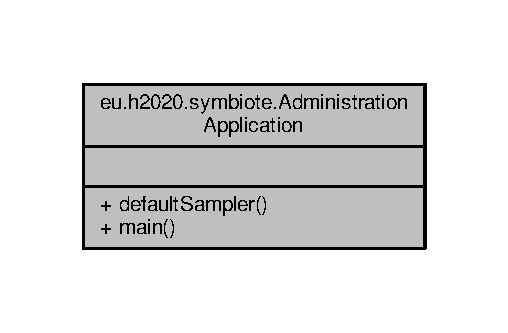
\includegraphics[width=244pt]{classeu_1_1h2020_1_1symbiote_1_1AdministrationApplication__coll__graph}
\end{center}
\end{figure}
\subsection*{Classes}
\begin{DoxyCompactItemize}
\item 
class {\bfseries C\+LR}
\end{DoxyCompactItemize}
\subsection*{Public Member Functions}
\begin{DoxyCompactItemize}
\item 
Always\+Sampler {\bfseries default\+Sampler} ()\hypertarget{classeu_1_1h2020_1_1symbiote_1_1AdministrationApplication_acb22f0581e401a988bae1d71fa5a2846}{}\label{classeu_1_1h2020_1_1symbiote_1_1AdministrationApplication_acb22f0581e401a988bae1d71fa5a2846}

\end{DoxyCompactItemize}
\subsection*{Static Public Member Functions}
\begin{DoxyCompactItemize}
\item 
static void {\bfseries main} (String\mbox{[}$\,$\mbox{]} args)\hypertarget{classeu_1_1h2020_1_1symbiote_1_1AdministrationApplication_aff5b1818698eef500f840eb62d696999}{}\label{classeu_1_1h2020_1_1symbiote_1_1AdministrationApplication_aff5b1818698eef500f840eb62d696999}

\end{DoxyCompactItemize}


\subsection{Detailed Description}
Administration module\textquotesingle{}s entry point. 

Administration is responsible for registering platforms by platform owners. It provides a web-\/based G\+UI for performing platform operations. 

The documentation for this class was generated from the following file\+:\begin{DoxyCompactItemize}
\item 
src/main/java/eu/h2020/symbiote/Administration\+Application.\+java\end{DoxyCompactItemize}

\hypertarget{classeu_1_1h2020_1_1symbiote_1_1controller_1_1Cpanel}{}\section{eu.\+h2020.\+symbiote.\+controller.\+Cpanel Class Reference}
\label{classeu_1_1h2020_1_1symbiote_1_1controller_1_1Cpanel}\index{eu.\+h2020.\+symbiote.\+controller.\+Cpanel@{eu.\+h2020.\+symbiote.\+controller.\+Cpanel}}


Collaboration diagram for eu.\+h2020.\+symbiote.\+controller.\+Cpanel\+:
\nopagebreak
\begin{figure}[H]
\begin{center}
\leavevmode
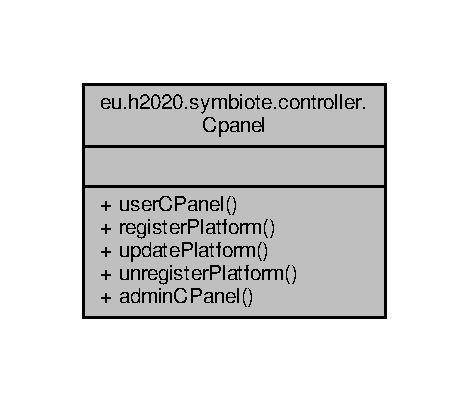
\includegraphics[width=225pt]{classeu_1_1h2020_1_1symbiote_1_1controller_1_1Cpanel__coll__graph}
\end{center}
\end{figure}
\subsection*{Public Member Functions}
\begin{DoxyCompactItemize}
\item 
String {\bfseries user\+C\+Panel} (Model model, Principal principal)\hypertarget{classeu_1_1h2020_1_1symbiote_1_1controller_1_1Cpanel_a009092cae8a35727082ffced5b0fcc81}{}\label{classeu_1_1h2020_1_1symbiote_1_1controller_1_1Cpanel_a009092cae8a35727082ffced5b0fcc81}

\item 
String {\bfseries register\+Platform} (@Valid \hyperlink{classeu_1_1h2020_1_1symbiote_1_1model_1_1Platform}{Platform} platform, Binding\+Result binding\+Result, Model model, Principal principal)\hypertarget{classeu_1_1h2020_1_1symbiote_1_1controller_1_1Cpanel_ab67932ffbb8960df71f5bbca270b23f4}{}\label{classeu_1_1h2020_1_1symbiote_1_1controller_1_1Cpanel_ab67932ffbb8960df71f5bbca270b23f4}

\item 
String {\bfseries update\+Platform} (@Valid \hyperlink{classeu_1_1h2020_1_1symbiote_1_1model_1_1Platform}{Platform} platform, Binding\+Result binding\+Result, Model model, Principal principal)\hypertarget{classeu_1_1h2020_1_1symbiote_1_1controller_1_1Cpanel_abd4d2749f0068279db583cf328b27426}{}\label{classeu_1_1h2020_1_1symbiote_1_1controller_1_1Cpanel_abd4d2749f0068279db583cf328b27426}

\item 
String {\bfseries unregister\+Platform} (Model model, Principal principal)\hypertarget{classeu_1_1h2020_1_1symbiote_1_1controller_1_1Cpanel_a7afae63cc7bb39aaaaf8e9d6ee87d03f}{}\label{classeu_1_1h2020_1_1symbiote_1_1controller_1_1Cpanel_a7afae63cc7bb39aaaaf8e9d6ee87d03f}

\item 
String {\bfseries admin\+C\+Panel} (Model model)\hypertarget{classeu_1_1h2020_1_1symbiote_1_1controller_1_1Cpanel_ad0f6fb280ef1ac2658fa3852ec8c6dd9}{}\label{classeu_1_1h2020_1_1symbiote_1_1controller_1_1Cpanel_ad0f6fb280ef1ac2658fa3852ec8c6dd9}

\end{DoxyCompactItemize}


The documentation for this class was generated from the following file\+:\begin{DoxyCompactItemize}
\item 
src/main/java/eu/h2020/symbiote/controllers/Cpanel.\+java\end{DoxyCompactItemize}

\hypertarget{classeu_1_1h2020_1_1symbiote_1_1communication_1_1EmptyConsumerReturnListener}{}\section{eu.\+h2020.\+symbiote.\+communication.\+Empty\+Consumer\+Return\+Listener Class Reference}
\label{classeu_1_1h2020_1_1symbiote_1_1communication_1_1EmptyConsumerReturnListener}\index{eu.\+h2020.\+symbiote.\+communication.\+Empty\+Consumer\+Return\+Listener@{eu.\+h2020.\+symbiote.\+communication.\+Empty\+Consumer\+Return\+Listener}}


Inheritance diagram for eu.\+h2020.\+symbiote.\+communication.\+Empty\+Consumer\+Return\+Listener\+:
\nopagebreak
\begin{figure}[H]
\begin{center}
\leavevmode
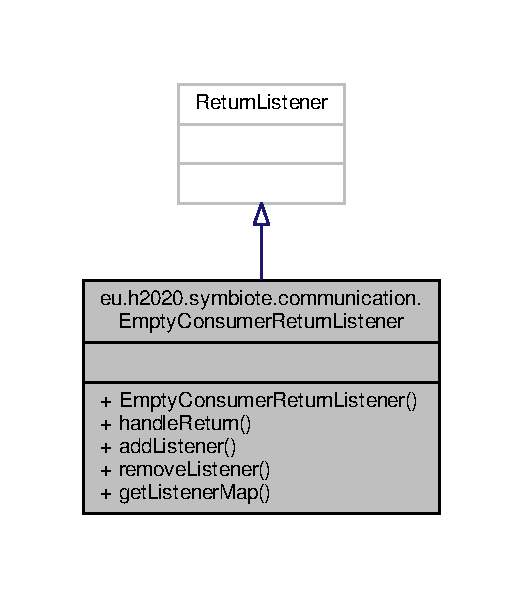
\includegraphics[width=251pt]{classeu_1_1h2020_1_1symbiote_1_1communication_1_1EmptyConsumerReturnListener__inherit__graph}
\end{center}
\end{figure}


Collaboration diagram for eu.\+h2020.\+symbiote.\+communication.\+Empty\+Consumer\+Return\+Listener\+:
\nopagebreak
\begin{figure}[H]
\begin{center}
\leavevmode
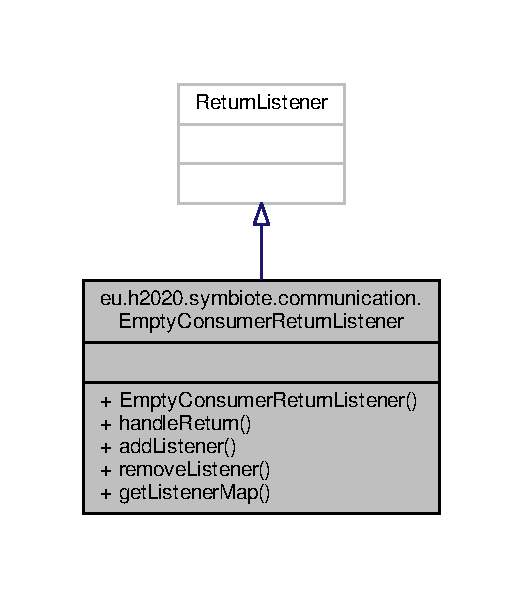
\includegraphics[width=251pt]{classeu_1_1h2020_1_1symbiote_1_1communication_1_1EmptyConsumerReturnListener__coll__graph}
\end{center}
\end{figure}
\subsection*{Public Member Functions}
\begin{DoxyCompactItemize}
\item 
\hyperlink{classeu_1_1h2020_1_1symbiote_1_1communication_1_1EmptyConsumerReturnListener_a9ec79d1d093e2380bf03fa1f76ce2261}{Empty\+Consumer\+Return\+Listener} ()
\item 
void \hyperlink{classeu_1_1h2020_1_1symbiote_1_1communication_1_1EmptyConsumerReturnListener_a612cd000e7188e6f05091e3f3673fb1d}{handle\+Return} (int reply\+Code, String reply\+Text, String exchange, String routing\+Key, A\+M\+Q\+P.\+Basic\+Properties properties, byte\mbox{[}$\,$\mbox{]} body)  throws I\+O\+Exception 
\item 
void \hyperlink{classeu_1_1h2020_1_1symbiote_1_1communication_1_1EmptyConsumerReturnListener_aaa1b35e4c336a029f118a19b9162e812}{add\+Listener} (String queue\+Name, String correlation\+Id, \hyperlink{interfaceeu_1_1h2020_1_1symbiote_1_1communication_1_1IRpcResponseListener}{I\+Rpc\+Response\+Listener} listener)
\item 
void \hyperlink{classeu_1_1h2020_1_1symbiote_1_1communication_1_1EmptyConsumerReturnListener_a89ad674c17d6304781ed91117aac0153}{remove\+Listener} (String queue\+Name, String correlation\+Id)
\item 
Map$<$ Pair, \hyperlink{interfaceeu_1_1h2020_1_1symbiote_1_1communication_1_1IRpcResponseListener}{I\+Rpc\+Response\+Listener} $>$ \hyperlink{classeu_1_1h2020_1_1symbiote_1_1communication_1_1EmptyConsumerReturnListener_afc62e8333afe576bc3a211195f7ade06}{get\+Listener\+Map} ()
\end{DoxyCompactItemize}


\subsection{Detailed Description}
Class responsible for handling R\+PC messages send to an exchange without bound consumers. 

When request is sent to an exchange without any consumers subscribed, it will not be buffered, but will disappear without any trace. Therefore, not only the request will not be served, but also caller will not get back any notification, since communication is done asynchronously. That\textquotesingle{}s where \hyperlink{classeu_1_1h2020_1_1symbiote_1_1communication_1_1EmptyConsumerReturnListener}{Empty\+Consumer\+Return\+Listener} comes to work. If it gets called by failing to deliver a mandatory message, it will notify the registered response listener that the request could not be served. 

\subsection{Constructor \& Destructor Documentation}
\index{eu\+::h2020\+::symbiote\+::communication\+::\+Empty\+Consumer\+Return\+Listener@{eu\+::h2020\+::symbiote\+::communication\+::\+Empty\+Consumer\+Return\+Listener}!Empty\+Consumer\+Return\+Listener@{Empty\+Consumer\+Return\+Listener}}
\index{Empty\+Consumer\+Return\+Listener@{Empty\+Consumer\+Return\+Listener}!eu\+::h2020\+::symbiote\+::communication\+::\+Empty\+Consumer\+Return\+Listener@{eu\+::h2020\+::symbiote\+::communication\+::\+Empty\+Consumer\+Return\+Listener}}
\subsubsection[{\texorpdfstring{Empty\+Consumer\+Return\+Listener()}{EmptyConsumerReturnListener()}}]{\setlength{\rightskip}{0pt plus 5cm}eu.\+h2020.\+symbiote.\+communication.\+Empty\+Consumer\+Return\+Listener.\+Empty\+Consumer\+Return\+Listener (
\begin{DoxyParamCaption}
{}
\end{DoxyParamCaption}
)}\hypertarget{classeu_1_1h2020_1_1symbiote_1_1communication_1_1EmptyConsumerReturnListener_a9ec79d1d093e2380bf03fa1f76ce2261}{}\label{classeu_1_1h2020_1_1symbiote_1_1communication_1_1EmptyConsumerReturnListener_a9ec79d1d093e2380bf03fa1f76ce2261}
Default empty constructor. 

\subsection{Member Function Documentation}
\index{eu\+::h2020\+::symbiote\+::communication\+::\+Empty\+Consumer\+Return\+Listener@{eu\+::h2020\+::symbiote\+::communication\+::\+Empty\+Consumer\+Return\+Listener}!add\+Listener@{add\+Listener}}
\index{add\+Listener@{add\+Listener}!eu\+::h2020\+::symbiote\+::communication\+::\+Empty\+Consumer\+Return\+Listener@{eu\+::h2020\+::symbiote\+::communication\+::\+Empty\+Consumer\+Return\+Listener}}
\subsubsection[{\texorpdfstring{add\+Listener(\+String queue\+Name, String correlation\+Id, I\+Rpc\+Response\+Listener listener)}{addListener(String queueName, String correlationId, IRpcResponseListener listener)}}]{\setlength{\rightskip}{0pt plus 5cm}void eu.\+h2020.\+symbiote.\+communication.\+Empty\+Consumer\+Return\+Listener.\+add\+Listener (
\begin{DoxyParamCaption}
\item[{String}]{queue\+Name, }
\item[{String}]{correlation\+Id, }
\item[{{\bf I\+Rpc\+Response\+Listener}}]{listener}
\end{DoxyParamCaption}
)}\hypertarget{classeu_1_1h2020_1_1symbiote_1_1communication_1_1EmptyConsumerReturnListener_aaa1b35e4c336a029f118a19b9162e812}{}\label{classeu_1_1h2020_1_1symbiote_1_1communication_1_1EmptyConsumerReturnListener_aaa1b35e4c336a029f118a19b9162e812}
Method used to register response listener for specified reply queue name and correlation ID.


\begin{DoxyParams}{Parameters}
{\em queue\+Name} & reply queue name to register listener for \\
\hline
{\em correlation\+Id} & correlation ID to register listener for \\
\hline
{\em listener} & response listener to register \\
\hline
\end{DoxyParams}
\index{eu\+::h2020\+::symbiote\+::communication\+::\+Empty\+Consumer\+Return\+Listener@{eu\+::h2020\+::symbiote\+::communication\+::\+Empty\+Consumer\+Return\+Listener}!get\+Listener\+Map@{get\+Listener\+Map}}
\index{get\+Listener\+Map@{get\+Listener\+Map}!eu\+::h2020\+::symbiote\+::communication\+::\+Empty\+Consumer\+Return\+Listener@{eu\+::h2020\+::symbiote\+::communication\+::\+Empty\+Consumer\+Return\+Listener}}
\subsubsection[{\texorpdfstring{get\+Listener\+Map()}{getListenerMap()}}]{\setlength{\rightskip}{0pt plus 5cm}Map$<$Pair, {\bf I\+Rpc\+Response\+Listener}$>$ eu.\+h2020.\+symbiote.\+communication.\+Empty\+Consumer\+Return\+Listener.\+get\+Listener\+Map (
\begin{DoxyParamCaption}
{}
\end{DoxyParamCaption}
)}\hypertarget{classeu_1_1h2020_1_1symbiote_1_1communication_1_1EmptyConsumerReturnListener_afc62e8333afe576bc3a211195f7ade06}{}\label{classeu_1_1h2020_1_1symbiote_1_1communication_1_1EmptyConsumerReturnListener_afc62e8333afe576bc3a211195f7ade06}
For the purpose of Unit Tests.

\begin{DoxyReturn}{Returns}
map of registered listeners 
\end{DoxyReturn}
\index{eu\+::h2020\+::symbiote\+::communication\+::\+Empty\+Consumer\+Return\+Listener@{eu\+::h2020\+::symbiote\+::communication\+::\+Empty\+Consumer\+Return\+Listener}!handle\+Return@{handle\+Return}}
\index{handle\+Return@{handle\+Return}!eu\+::h2020\+::symbiote\+::communication\+::\+Empty\+Consumer\+Return\+Listener@{eu\+::h2020\+::symbiote\+::communication\+::\+Empty\+Consumer\+Return\+Listener}}
\subsubsection[{\texorpdfstring{handle\+Return(int reply\+Code, String reply\+Text, String exchange, String routing\+Key, A\+M\+Q\+P.\+Basic\+Properties properties, byte[] body)}{handleReturn(int replyCode, String replyText, String exchange, String routingKey, AMQP.BasicProperties properties, byte[] body)}}]{\setlength{\rightskip}{0pt plus 5cm}void eu.\+h2020.\+symbiote.\+communication.\+Empty\+Consumer\+Return\+Listener.\+handle\+Return (
\begin{DoxyParamCaption}
\item[{int}]{reply\+Code, }
\item[{String}]{reply\+Text, }
\item[{String}]{exchange, }
\item[{String}]{routing\+Key, }
\item[{A\+M\+Q\+P.\+Basic\+Properties}]{properties, }
\item[{byte\mbox{[}$\,$\mbox{]}}]{body}
\end{DoxyParamCaption}
) throws I\+O\+Exception}\hypertarget{classeu_1_1h2020_1_1symbiote_1_1communication_1_1EmptyConsumerReturnListener_a612cd000e7188e6f05091e3f3673fb1d}{}\label{classeu_1_1h2020_1_1symbiote_1_1communication_1_1EmptyConsumerReturnListener_a612cd000e7188e6f05091e3f3673fb1d}
Implementation of handling return message from Rabbit\+MQ. 

When a mandatory message is to be sent, its response listener is registered using \{\hyperlink{classeu_1_1h2020_1_1symbiote_1_1communication_1_1EmptyConsumerReturnListener_aaa1b35e4c336a029f118a19b9162e812}{add\+Listener(\+String, String, I\+Rpc\+Response\+Listener)}\} method, using reply queue name and correlation ID as key. When the handle\+Return method is called, it checks the message\textquotesingle{}s reply queue name and correlation ID to find out if the response listener has been registered for it. If so, it fires it with proper response message (that is status 500 -\/ Internal Server Error, and empty body). 

When message was handled succesfully by consumer, its response listener is unregistered from \hyperlink{classeu_1_1h2020_1_1symbiote_1_1communication_1_1EmptyConsumerReturnListener}{Empty\+Consumer\+Return\+Listener}.


\begin{DoxyParams}{Parameters}
{\em reply\+Code} & irrelevant for this implementation of Return\+Listener \\
\hline
{\em reply\+Text} & irrelevant for this implementation of Return\+Listener \\
\hline
{\em exchange} & irrelevant for this implementation of Return\+Listener \\
\hline
{\em routing\+Key} & irrelevant for this implementation of Return\+Listener \\
\hline
{\em properties} & properties object that was sent with the message; it should contain both reply\+To and correlation\+Id parameters \\
\hline
{\em body} & irrelevant for this implementation of Return\+Listener \\
\hline
\end{DoxyParams}

\begin{DoxyExceptions}{Exceptions}
{\em I\+O\+Exception} & \\
\hline
\end{DoxyExceptions}
\index{eu\+::h2020\+::symbiote\+::communication\+::\+Empty\+Consumer\+Return\+Listener@{eu\+::h2020\+::symbiote\+::communication\+::\+Empty\+Consumer\+Return\+Listener}!remove\+Listener@{remove\+Listener}}
\index{remove\+Listener@{remove\+Listener}!eu\+::h2020\+::symbiote\+::communication\+::\+Empty\+Consumer\+Return\+Listener@{eu\+::h2020\+::symbiote\+::communication\+::\+Empty\+Consumer\+Return\+Listener}}
\subsubsection[{\texorpdfstring{remove\+Listener(\+String queue\+Name, String correlation\+Id)}{removeListener(String queueName, String correlationId)}}]{\setlength{\rightskip}{0pt plus 5cm}void eu.\+h2020.\+symbiote.\+communication.\+Empty\+Consumer\+Return\+Listener.\+remove\+Listener (
\begin{DoxyParamCaption}
\item[{String}]{queue\+Name, }
\item[{String}]{correlation\+Id}
\end{DoxyParamCaption}
)}\hypertarget{classeu_1_1h2020_1_1symbiote_1_1communication_1_1EmptyConsumerReturnListener_a89ad674c17d6304781ed91117aac0153}{}\label{classeu_1_1h2020_1_1symbiote_1_1communication_1_1EmptyConsumerReturnListener_a89ad674c17d6304781ed91117aac0153}
Method used to unregister response listener for specified reply queue name and correlation ID.


\begin{DoxyParams}{Parameters}
{\em queue\+Name} & reply queue name to unregister listener for \\
\hline
{\em correlation\+Id} & correlation ID to unregister listener for \\
\hline
\end{DoxyParams}


The documentation for this class was generated from the following file\+:\begin{DoxyCompactItemize}
\item 
src/main/java/eu/h2020/symbiote/communication/Empty\+Consumer\+Return\+Listener.\+java\end{DoxyCompactItemize}

\hypertarget{interfaceeu_1_1h2020_1_1symbiote_1_1communication_1_1IRpcResponseListener}{}\section{eu.\+h2020.\+symbiote.\+communication.\+I\+Rpc\+Response\+Listener Interface Reference}
\label{interfaceeu_1_1h2020_1_1symbiote_1_1communication_1_1IRpcResponseListener}\index{eu.\+h2020.\+symbiote.\+communication.\+I\+Rpc\+Response\+Listener@{eu.\+h2020.\+symbiote.\+communication.\+I\+Rpc\+Response\+Listener}}


Collaboration diagram for eu.\+h2020.\+symbiote.\+communication.\+I\+Rpc\+Response\+Listener\+:
\nopagebreak
\begin{figure}[H]
\begin{center}
\leavevmode
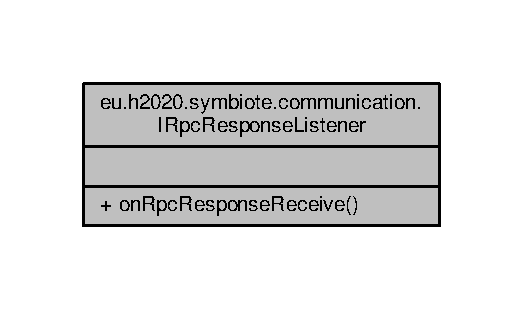
\includegraphics[width=251pt]{interfaceeu_1_1h2020_1_1symbiote_1_1communication_1_1IRpcResponseListener__coll__graph}
\end{center}
\end{figure}
\subsection*{Public Member Functions}
\begin{DoxyCompactItemize}
\item 
void \hyperlink{interfaceeu_1_1h2020_1_1symbiote_1_1communication_1_1IRpcResponseListener_ad9d4acebc86817e20f4ce3e07aeee8ae}{on\+Rpc\+Response\+Receive} (\hyperlink{classeu_1_1h2020_1_1symbiote_1_1model_1_1RpcPlatformResponse}{Rpc\+Platform\+Response} rpc\+Platform\+Response)
\end{DoxyCompactItemize}


\subsection{Detailed Description}
Interface used as a response listener for R\+PC Rabbit\+MQ communication. 

When a message is sent using asynchronous R\+PC call, it needs to pass listener that waits for the response. 

\subsection{Member Function Documentation}
\index{eu\+::h2020\+::symbiote\+::communication\+::\+I\+Rpc\+Response\+Listener@{eu\+::h2020\+::symbiote\+::communication\+::\+I\+Rpc\+Response\+Listener}!on\+Rpc\+Response\+Receive@{on\+Rpc\+Response\+Receive}}
\index{on\+Rpc\+Response\+Receive@{on\+Rpc\+Response\+Receive}!eu\+::h2020\+::symbiote\+::communication\+::\+I\+Rpc\+Response\+Listener@{eu\+::h2020\+::symbiote\+::communication\+::\+I\+Rpc\+Response\+Listener}}
\subsubsection[{\texorpdfstring{on\+Rpc\+Response\+Receive(\+Rpc\+Platform\+Response rpc\+Platform\+Response)}{onRpcResponseReceive(RpcPlatformResponse rpcPlatformResponse)}}]{\setlength{\rightskip}{0pt plus 5cm}void eu.\+h2020.\+symbiote.\+communication.\+I\+Rpc\+Response\+Listener.\+on\+Rpc\+Response\+Receive (
\begin{DoxyParamCaption}
\item[{{\bf Rpc\+Platform\+Response}}]{rpc\+Platform\+Response}
\end{DoxyParamCaption}
)}\hypertarget{interfaceeu_1_1h2020_1_1symbiote_1_1communication_1_1IRpcResponseListener_ad9d4acebc86817e20f4ce3e07aeee8ae}{}\label{interfaceeu_1_1h2020_1_1symbiote_1_1communication_1_1IRpcResponseListener_ad9d4acebc86817e20f4ce3e07aeee8ae}
When the response to sent request is available, this method is called, passing response object as parameter.


\begin{DoxyParams}{Parameters}
{\em rpc\+Platform\+Response} & R\+PC response object \\
\hline
\end{DoxyParams}


The documentation for this interface was generated from the following file\+:\begin{DoxyCompactItemize}
\item 
src/main/java/eu/h2020/symbiote/communication/I\+Rpc\+Response\+Listener.\+java\end{DoxyCompactItemize}

\hypertarget{classeu_1_1h2020_1_1symbiote_1_1MvcConfig}{}\section{eu.\+h2020.\+symbiote.\+Mvc\+Config Class Reference}
\label{classeu_1_1h2020_1_1symbiote_1_1MvcConfig}\index{eu.\+h2020.\+symbiote.\+Mvc\+Config@{eu.\+h2020.\+symbiote.\+Mvc\+Config}}


Inheritance diagram for eu.\+h2020.\+symbiote.\+Mvc\+Config\+:
\nopagebreak
\begin{figure}[H]
\begin{center}
\leavevmode
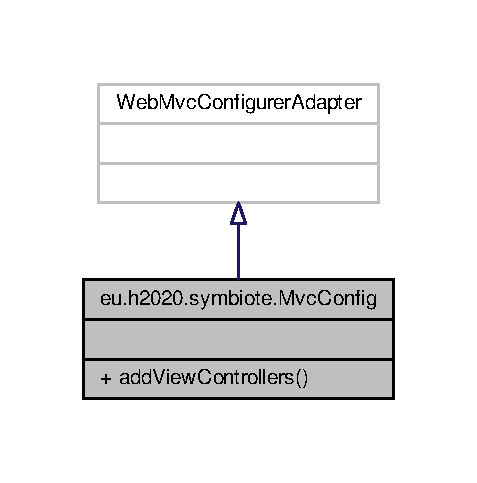
\includegraphics[width=229pt]{classeu_1_1h2020_1_1symbiote_1_1MvcConfig__inherit__graph}
\end{center}
\end{figure}


Collaboration diagram for eu.\+h2020.\+symbiote.\+Mvc\+Config\+:
\nopagebreak
\begin{figure}[H]
\begin{center}
\leavevmode
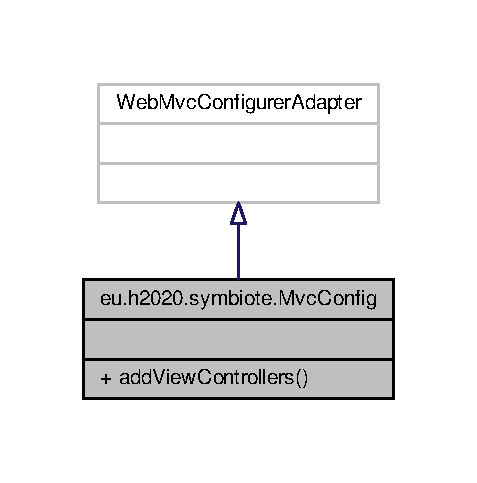
\includegraphics[width=229pt]{classeu_1_1h2020_1_1symbiote_1_1MvcConfig__coll__graph}
\end{center}
\end{figure}
\subsection*{Public Member Functions}
\begin{DoxyCompactItemize}
\item 
void {\bfseries add\+View\+Controllers} (View\+Controller\+Registry registry)\hypertarget{classeu_1_1h2020_1_1symbiote_1_1MvcConfig_a8ab502c0631464766b89de95f1c235f0}{}\label{classeu_1_1h2020_1_1symbiote_1_1MvcConfig_a8ab502c0631464766b89de95f1c235f0}

\end{DoxyCompactItemize}


The documentation for this class was generated from the following file\+:\begin{DoxyCompactItemize}
\item 
src/main/java/eu/h2020/symbiote/Mvc\+Config.\+java\end{DoxyCompactItemize}

\hypertarget{classeu_1_1h2020_1_1symbiote_1_1model_1_1Platform}{}\section{eu.\+h2020.\+symbiote.\+model.\+Platform Class Reference}
\label{classeu_1_1h2020_1_1symbiote_1_1model_1_1Platform}\index{eu.\+h2020.\+symbiote.\+model.\+Platform@{eu.\+h2020.\+symbiote.\+model.\+Platform}}


Collaboration diagram for eu.\+h2020.\+symbiote.\+model.\+Platform\+:
\nopagebreak
\begin{figure}[H]
\begin{center}
\leavevmode
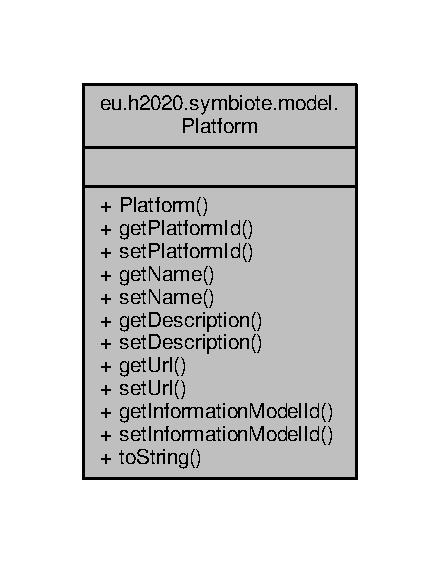
\includegraphics[width=211pt]{classeu_1_1h2020_1_1symbiote_1_1model_1_1Platform__coll__graph}
\end{center}
\end{figure}
\subsection*{Public Member Functions}
\begin{DoxyCompactItemize}
\item 
\hyperlink{classeu_1_1h2020_1_1symbiote_1_1model_1_1Platform_a30253edbb49569262e02dc24c516ed6d}{Platform} ()
\item 
String {\bfseries get\+Platform\+Id} ()\hypertarget{classeu_1_1h2020_1_1symbiote_1_1model_1_1Platform_a2a09b94af05846adcf58f6405f0b1fdc}{}\label{classeu_1_1h2020_1_1symbiote_1_1model_1_1Platform_a2a09b94af05846adcf58f6405f0b1fdc}

\item 
void {\bfseries set\+Platform\+Id} (String platform\+Id)\hypertarget{classeu_1_1h2020_1_1symbiote_1_1model_1_1Platform_a3d9e886790d506f713e997f3c587e8ac}{}\label{classeu_1_1h2020_1_1symbiote_1_1model_1_1Platform_a3d9e886790d506f713e997f3c587e8ac}

\item 
String {\bfseries get\+Name} ()\hypertarget{classeu_1_1h2020_1_1symbiote_1_1model_1_1Platform_a9d39e85c470888c7043448f2eb059325}{}\label{classeu_1_1h2020_1_1symbiote_1_1model_1_1Platform_a9d39e85c470888c7043448f2eb059325}

\item 
void {\bfseries set\+Name} (String name)\hypertarget{classeu_1_1h2020_1_1symbiote_1_1model_1_1Platform_af4d5506c08659b3d71dcc8bf69c743ce}{}\label{classeu_1_1h2020_1_1symbiote_1_1model_1_1Platform_af4d5506c08659b3d71dcc8bf69c743ce}

\item 
String {\bfseries get\+Description} ()\hypertarget{classeu_1_1h2020_1_1symbiote_1_1model_1_1Platform_ad4a8d6cbb5ed57e241f783c512f052d9}{}\label{classeu_1_1h2020_1_1symbiote_1_1model_1_1Platform_ad4a8d6cbb5ed57e241f783c512f052d9}

\item 
void {\bfseries set\+Description} (String description)\hypertarget{classeu_1_1h2020_1_1symbiote_1_1model_1_1Platform_a9ec81f09b9fcd25ae264618591992cb2}{}\label{classeu_1_1h2020_1_1symbiote_1_1model_1_1Platform_a9ec81f09b9fcd25ae264618591992cb2}

\item 
String {\bfseries get\+Url} ()\hypertarget{classeu_1_1h2020_1_1symbiote_1_1model_1_1Platform_a4ca440b89e37c323dcb812ef07cfb66a}{}\label{classeu_1_1h2020_1_1symbiote_1_1model_1_1Platform_a4ca440b89e37c323dcb812ef07cfb66a}

\item 
void {\bfseries set\+Url} (String url)\hypertarget{classeu_1_1h2020_1_1symbiote_1_1model_1_1Platform_ac4d39a74475da2c2318cfd5e3667a5a1}{}\label{classeu_1_1h2020_1_1symbiote_1_1model_1_1Platform_ac4d39a74475da2c2318cfd5e3667a5a1}

\item 
String {\bfseries get\+Information\+Model\+Id} ()\hypertarget{classeu_1_1h2020_1_1symbiote_1_1model_1_1Platform_a799a5bb8e0665457c4b8bfd2b34c9b3c}{}\label{classeu_1_1h2020_1_1symbiote_1_1model_1_1Platform_a799a5bb8e0665457c4b8bfd2b34c9b3c}

\item 
void {\bfseries set\+Information\+Model\+Id} (String information\+Model\+Id)\hypertarget{classeu_1_1h2020_1_1symbiote_1_1model_1_1Platform_ae3e1cb93bcb289d575f215990d7e9499}{}\label{classeu_1_1h2020_1_1symbiote_1_1model_1_1Platform_ae3e1cb93bcb289d575f215990d7e9499}

\item 
String {\bfseries to\+String} ()\hypertarget{classeu_1_1h2020_1_1symbiote_1_1model_1_1Platform_a934fa4d3de67f063c2ccd5f76c155ec8}{}\label{classeu_1_1h2020_1_1symbiote_1_1model_1_1Platform_a934fa4d3de67f063c2ccd5f76c155ec8}

\end{DoxyCompactItemize}


\subsection{Detailed Description}
P\+O\+JO describing a platform. 

\subsection{Constructor \& Destructor Documentation}
\index{eu\+::h2020\+::symbiote\+::model\+::\+Platform@{eu\+::h2020\+::symbiote\+::model\+::\+Platform}!Platform@{Platform}}
\index{Platform@{Platform}!eu\+::h2020\+::symbiote\+::model\+::\+Platform@{eu\+::h2020\+::symbiote\+::model\+::\+Platform}}
\subsubsection[{\texorpdfstring{Platform()}{Platform()}}]{\setlength{\rightskip}{0pt plus 5cm}eu.\+h2020.\+symbiote.\+model.\+Platform.\+Platform (
\begin{DoxyParamCaption}
{}
\end{DoxyParamCaption}
)}\hypertarget{classeu_1_1h2020_1_1symbiote_1_1model_1_1Platform_a30253edbb49569262e02dc24c516ed6d}{}\label{classeu_1_1h2020_1_1symbiote_1_1model_1_1Platform_a30253edbb49569262e02dc24c516ed6d}
Default empty constructor. 

The documentation for this class was generated from the following file\+:\begin{DoxyCompactItemize}
\item 
src/main/java/eu/h2020/symbiote/model/Platform.\+java\end{DoxyCompactItemize}

\hypertarget{interfaceeu_1_1h2020_1_1symbiote_1_1repository_1_1PlatformRepository}{}\section{eu.\+h2020.\+symbiote.\+repository.\+Platform\+Repository Interface Reference}
\label{interfaceeu_1_1h2020_1_1symbiote_1_1repository_1_1PlatformRepository}\index{eu.\+h2020.\+symbiote.\+repository.\+Platform\+Repository@{eu.\+h2020.\+symbiote.\+repository.\+Platform\+Repository}}


Inheritance diagram for eu.\+h2020.\+symbiote.\+repository.\+Platform\+Repository\+:
\nopagebreak
\begin{figure}[H]
\begin{center}
\leavevmode
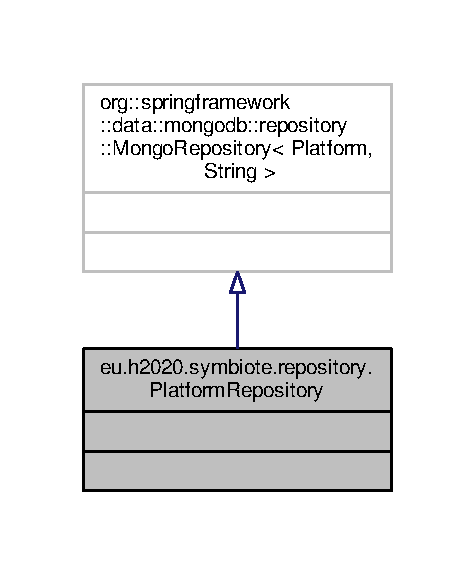
\includegraphics[width=228pt]{interfaceeu_1_1h2020_1_1symbiote_1_1repository_1_1PlatformRepository__inherit__graph}
\end{center}
\end{figure}


Collaboration diagram for eu.\+h2020.\+symbiote.\+repository.\+Platform\+Repository\+:
\nopagebreak
\begin{figure}[H]
\begin{center}
\leavevmode
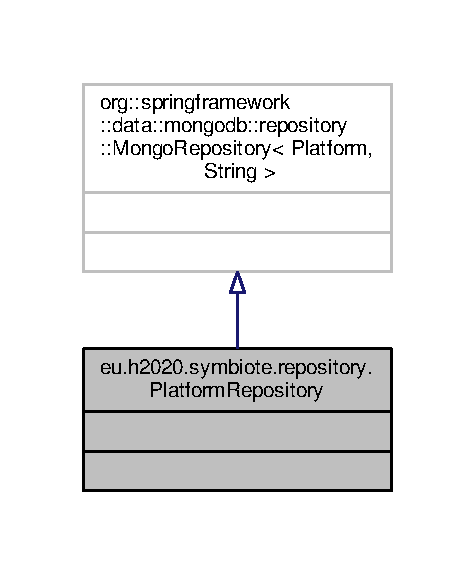
\includegraphics[width=228pt]{interfaceeu_1_1h2020_1_1symbiote_1_1repository_1_1PlatformRepository__coll__graph}
\end{center}
\end{figure}


\subsection{Detailed Description}
Created by mateuszl on 09.\+01.\+2017. 

The documentation for this interface was generated from the following file\+:\begin{DoxyCompactItemize}
\item 
src/main/java/eu/h2020/symbiote/repository/Platform\+Repository.\+java\end{DoxyCompactItemize}

\hypertarget{classeu_1_1h2020_1_1symbiote_1_1communication_1_1RabbitManager}{}\section{eu.\+h2020.\+symbiote.\+communication.\+Rabbit\+Manager Class Reference}
\label{classeu_1_1h2020_1_1symbiote_1_1communication_1_1RabbitManager}\index{eu.\+h2020.\+symbiote.\+communication.\+Rabbit\+Manager@{eu.\+h2020.\+symbiote.\+communication.\+Rabbit\+Manager}}


Collaboration diagram for eu.\+h2020.\+symbiote.\+communication.\+Rabbit\+Manager\+:
\nopagebreak
\begin{figure}[H]
\begin{center}
\leavevmode
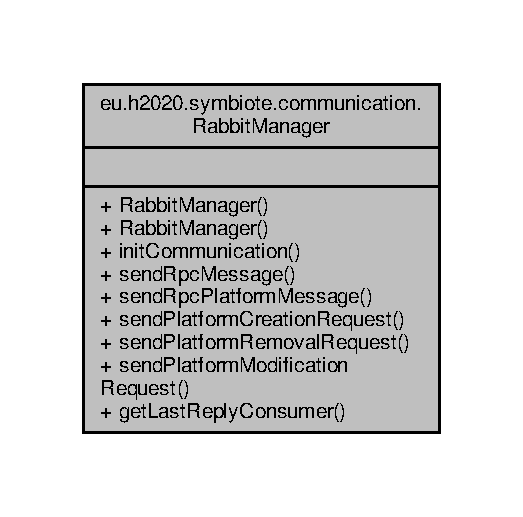
\includegraphics[width=251pt]{classeu_1_1h2020_1_1symbiote_1_1communication_1_1RabbitManager__coll__graph}
\end{center}
\end{figure}
\subsection*{Public Member Functions}
\begin{DoxyCompactItemize}
\item 
\hyperlink{classeu_1_1h2020_1_1symbiote_1_1communication_1_1RabbitManager_af32aa97329fd60a0c4d158d13a261b30}{Rabbit\+Manager} ()
\item 
\hyperlink{classeu_1_1h2020_1_1symbiote_1_1communication_1_1RabbitManager_add62f0a65b573c741e8cf0e1bbc44a44}{Rabbit\+Manager} (\hyperlink{classeu_1_1h2020_1_1symbiote_1_1communication_1_1EmptyConsumerReturnListener}{Empty\+Consumer\+Return\+Listener} empty\+Consumer\+Return\+Listener, Channel channel)
\item 
void \hyperlink{classeu_1_1h2020_1_1symbiote_1_1communication_1_1RabbitManager_a30abf6a670122eb22a8105a206858616}{init\+Communication} ()
\item 
void \hyperlink{classeu_1_1h2020_1_1symbiote_1_1communication_1_1RabbitManager_a200f6aba21764770f8526f0682b08f1c}{send\+Rpc\+Message} (String exchange\+Name, String routing\+Key, String message, \hyperlink{interfaceeu_1_1h2020_1_1symbiote_1_1communication_1_1IRpcResponseListener}{I\+Rpc\+Response\+Listener} response\+Listener)
\item 
void \hyperlink{classeu_1_1h2020_1_1symbiote_1_1communication_1_1RabbitManager_a9dd2b250640a13346fabfba81ae22a07}{send\+Rpc\+Platform\+Message} (String exchange\+Name, String routing\+Key, \hyperlink{classeu_1_1h2020_1_1symbiote_1_1model_1_1Platform}{Platform} platform, \hyperlink{interfaceeu_1_1h2020_1_1symbiote_1_1communication_1_1IRpcResponseListener}{I\+Rpc\+Response\+Listener} response\+Listener)
\item 
void \hyperlink{classeu_1_1h2020_1_1symbiote_1_1communication_1_1RabbitManager_ac960f5c05843849848d650e49ef25ae9}{send\+Platform\+Creation\+Request} (\hyperlink{classeu_1_1h2020_1_1symbiote_1_1model_1_1Platform}{Platform} platform, \hyperlink{interfaceeu_1_1h2020_1_1symbiote_1_1communication_1_1IRpcResponseListener}{I\+Rpc\+Response\+Listener} listener)
\item 
void \hyperlink{classeu_1_1h2020_1_1symbiote_1_1communication_1_1RabbitManager_a7e730a2a9c5d62e5d3ff99fe28e23384}{send\+Platform\+Removal\+Request} (\hyperlink{classeu_1_1h2020_1_1symbiote_1_1model_1_1Platform}{Platform} platform, \hyperlink{interfaceeu_1_1h2020_1_1symbiote_1_1communication_1_1IRpcResponseListener}{I\+Rpc\+Response\+Listener} listener)
\item 
void \hyperlink{classeu_1_1h2020_1_1symbiote_1_1communication_1_1RabbitManager_a0ffb60c722cea85703dabfa6dbd6f18e}{send\+Platform\+Modification\+Request} (\hyperlink{classeu_1_1h2020_1_1symbiote_1_1model_1_1Platform}{Platform} platform, \hyperlink{interfaceeu_1_1h2020_1_1symbiote_1_1communication_1_1IRpcResponseListener}{I\+Rpc\+Response\+Listener} listener)
\item 
\hyperlink{classeu_1_1h2020_1_1symbiote_1_1communication_1_1ReplyConsumer}{Reply\+Consumer} \hyperlink{classeu_1_1h2020_1_1symbiote_1_1communication_1_1RabbitManager_a2b34a47ec1e4a0e359f81e81f8d8b693}{get\+Last\+Reply\+Consumer} ()
\end{DoxyCompactItemize}


\subsection{Detailed Description}
Class used for all internal communication using Rabbit\+MQ A\+M\+QP implementation. It works as a Spring Bean, and should be used via autowiring. 

\hyperlink{classeu_1_1h2020_1_1symbiote_1_1communication_1_1RabbitManager}{Rabbit\+Manager} uses properties taken from Core\+Config\+Server to set up communication (exchange parameters, routing keys etc.) 

\subsection{Constructor \& Destructor Documentation}
\index{eu\+::h2020\+::symbiote\+::communication\+::\+Rabbit\+Manager@{eu\+::h2020\+::symbiote\+::communication\+::\+Rabbit\+Manager}!Rabbit\+Manager@{Rabbit\+Manager}}
\index{Rabbit\+Manager@{Rabbit\+Manager}!eu\+::h2020\+::symbiote\+::communication\+::\+Rabbit\+Manager@{eu\+::h2020\+::symbiote\+::communication\+::\+Rabbit\+Manager}}
\subsubsection[{\texorpdfstring{Rabbit\+Manager()}{RabbitManager()}}]{\setlength{\rightskip}{0pt plus 5cm}eu.\+h2020.\+symbiote.\+communication.\+Rabbit\+Manager.\+Rabbit\+Manager (
\begin{DoxyParamCaption}
{}
\end{DoxyParamCaption}
)}\hypertarget{classeu_1_1h2020_1_1symbiote_1_1communication_1_1RabbitManager_af32aa97329fd60a0c4d158d13a261b30}{}\label{classeu_1_1h2020_1_1symbiote_1_1communication_1_1RabbitManager_af32aa97329fd60a0c4d158d13a261b30}
Default, empty constructor. \index{eu\+::h2020\+::symbiote\+::communication\+::\+Rabbit\+Manager@{eu\+::h2020\+::symbiote\+::communication\+::\+Rabbit\+Manager}!Rabbit\+Manager@{Rabbit\+Manager}}
\index{Rabbit\+Manager@{Rabbit\+Manager}!eu\+::h2020\+::symbiote\+::communication\+::\+Rabbit\+Manager@{eu\+::h2020\+::symbiote\+::communication\+::\+Rabbit\+Manager}}
\subsubsection[{\texorpdfstring{Rabbit\+Manager(\+Empty\+Consumer\+Return\+Listener empty\+Consumer\+Return\+Listener, Channel channel)}{RabbitManager(EmptyConsumerReturnListener emptyConsumerReturnListener, Channel channel)}}]{\setlength{\rightskip}{0pt plus 5cm}eu.\+h2020.\+symbiote.\+communication.\+Rabbit\+Manager.\+Rabbit\+Manager (
\begin{DoxyParamCaption}
\item[{{\bf Empty\+Consumer\+Return\+Listener}}]{empty\+Consumer\+Return\+Listener, }
\item[{Channel}]{channel}
\end{DoxyParamCaption}
)}\hypertarget{classeu_1_1h2020_1_1symbiote_1_1communication_1_1RabbitManager_add62f0a65b573c741e8cf0e1bbc44a44}{}\label{classeu_1_1h2020_1_1symbiote_1_1communication_1_1RabbitManager_add62f0a65b573c741e8cf0e1bbc44a44}
Constructor used only when doing Unit Tests. Used to pass mocked instance of empty\+Consumer\+Return\+Listener.


\begin{DoxyParams}{Parameters}
{\em empty\+Consumer\+Return\+Listener} & instance of listener handling empty consumer messages \\
\hline
{\em channel} & rabbit channel \\
\hline
\end{DoxyParams}


\subsection{Member Function Documentation}
\index{eu\+::h2020\+::symbiote\+::communication\+::\+Rabbit\+Manager@{eu\+::h2020\+::symbiote\+::communication\+::\+Rabbit\+Manager}!get\+Last\+Reply\+Consumer@{get\+Last\+Reply\+Consumer}}
\index{get\+Last\+Reply\+Consumer@{get\+Last\+Reply\+Consumer}!eu\+::h2020\+::symbiote\+::communication\+::\+Rabbit\+Manager@{eu\+::h2020\+::symbiote\+::communication\+::\+Rabbit\+Manager}}
\subsubsection[{\texorpdfstring{get\+Last\+Reply\+Consumer()}{getLastReplyConsumer()}}]{\setlength{\rightskip}{0pt plus 5cm}{\bf Reply\+Consumer} eu.\+h2020.\+symbiote.\+communication.\+Rabbit\+Manager.\+get\+Last\+Reply\+Consumer (
\begin{DoxyParamCaption}
{}
\end{DoxyParamCaption}
)}\hypertarget{classeu_1_1h2020_1_1symbiote_1_1communication_1_1RabbitManager_a2b34a47ec1e4a0e359f81e81f8d8b693}{}\label{classeu_1_1h2020_1_1symbiote_1_1communication_1_1RabbitManager_a2b34a47ec1e4a0e359f81e81f8d8b693}
Method used only when doing unit tests.

\begin{DoxyReturn}{Returns}
Last created reply consumer 
\end{DoxyReturn}
\index{eu\+::h2020\+::symbiote\+::communication\+::\+Rabbit\+Manager@{eu\+::h2020\+::symbiote\+::communication\+::\+Rabbit\+Manager}!init\+Communication@{init\+Communication}}
\index{init\+Communication@{init\+Communication}!eu\+::h2020\+::symbiote\+::communication\+::\+Rabbit\+Manager@{eu\+::h2020\+::symbiote\+::communication\+::\+Rabbit\+Manager}}
\subsubsection[{\texorpdfstring{init\+Communication()}{initCommunication()}}]{\setlength{\rightskip}{0pt plus 5cm}void eu.\+h2020.\+symbiote.\+communication.\+Rabbit\+Manager.\+init\+Communication (
\begin{DoxyParamCaption}
{}
\end{DoxyParamCaption}
)}\hypertarget{classeu_1_1h2020_1_1symbiote_1_1communication_1_1RabbitManager_a30abf6a670122eb22a8105a206858616}{}\label{classeu_1_1h2020_1_1symbiote_1_1communication_1_1RabbitManager_a30abf6a670122eb22a8105a206858616}
Method used to initialise Rabbit\+MQ connection and declare all required exchanges. This method should be called once, after bean initialization (so that properties from Core\+Config\+Server are obtained), but before using \hyperlink{classeu_1_1h2020_1_1symbiote_1_1communication_1_1RabbitManager}{Rabbit\+Manager} to send any message. \index{eu\+::h2020\+::symbiote\+::communication\+::\+Rabbit\+Manager@{eu\+::h2020\+::symbiote\+::communication\+::\+Rabbit\+Manager}!send\+Platform\+Creation\+Request@{send\+Platform\+Creation\+Request}}
\index{send\+Platform\+Creation\+Request@{send\+Platform\+Creation\+Request}!eu\+::h2020\+::symbiote\+::communication\+::\+Rabbit\+Manager@{eu\+::h2020\+::symbiote\+::communication\+::\+Rabbit\+Manager}}
\subsubsection[{\texorpdfstring{send\+Platform\+Creation\+Request(\+Platform platform, I\+Rpc\+Response\+Listener listener)}{sendPlatformCreationRequest(Platform platform, IRpcResponseListener listener)}}]{\setlength{\rightskip}{0pt plus 5cm}void eu.\+h2020.\+symbiote.\+communication.\+Rabbit\+Manager.\+send\+Platform\+Creation\+Request (
\begin{DoxyParamCaption}
\item[{{\bf Platform}}]{platform, }
\item[{{\bf I\+Rpc\+Response\+Listener}}]{listener}
\end{DoxyParamCaption}
)}\hypertarget{classeu_1_1h2020_1_1symbiote_1_1communication_1_1RabbitManager_ac960f5c05843849848d650e49ef25ae9}{}\label{classeu_1_1h2020_1_1symbiote_1_1communication_1_1RabbitManager_ac960f5c05843849848d650e49ef25ae9}
Method used to send R\+PC request to create platform.


\begin{DoxyParams}{Parameters}
{\em platform} & platform to be created \\
\hline
{\em listener} & listener for rpc response \\
\hline
\end{DoxyParams}
\index{eu\+::h2020\+::symbiote\+::communication\+::\+Rabbit\+Manager@{eu\+::h2020\+::symbiote\+::communication\+::\+Rabbit\+Manager}!send\+Platform\+Modification\+Request@{send\+Platform\+Modification\+Request}}
\index{send\+Platform\+Modification\+Request@{send\+Platform\+Modification\+Request}!eu\+::h2020\+::symbiote\+::communication\+::\+Rabbit\+Manager@{eu\+::h2020\+::symbiote\+::communication\+::\+Rabbit\+Manager}}
\subsubsection[{\texorpdfstring{send\+Platform\+Modification\+Request(\+Platform platform, I\+Rpc\+Response\+Listener listener)}{sendPlatformModificationRequest(Platform platform, IRpcResponseListener listener)}}]{\setlength{\rightskip}{0pt plus 5cm}void eu.\+h2020.\+symbiote.\+communication.\+Rabbit\+Manager.\+send\+Platform\+Modification\+Request (
\begin{DoxyParamCaption}
\item[{{\bf Platform}}]{platform, }
\item[{{\bf I\+Rpc\+Response\+Listener}}]{listener}
\end{DoxyParamCaption}
)}\hypertarget{classeu_1_1h2020_1_1symbiote_1_1communication_1_1RabbitManager_a0ffb60c722cea85703dabfa6dbd6f18e}{}\label{classeu_1_1h2020_1_1symbiote_1_1communication_1_1RabbitManager_a0ffb60c722cea85703dabfa6dbd6f18e}
Method used to send R\+PC request to modify platform.


\begin{DoxyParams}{Parameters}
{\em platform} & platform to be modified \\
\hline
{\em listener} & listener for rpc response \\
\hline
\end{DoxyParams}
\index{eu\+::h2020\+::symbiote\+::communication\+::\+Rabbit\+Manager@{eu\+::h2020\+::symbiote\+::communication\+::\+Rabbit\+Manager}!send\+Platform\+Removal\+Request@{send\+Platform\+Removal\+Request}}
\index{send\+Platform\+Removal\+Request@{send\+Platform\+Removal\+Request}!eu\+::h2020\+::symbiote\+::communication\+::\+Rabbit\+Manager@{eu\+::h2020\+::symbiote\+::communication\+::\+Rabbit\+Manager}}
\subsubsection[{\texorpdfstring{send\+Platform\+Removal\+Request(\+Platform platform, I\+Rpc\+Response\+Listener listener)}{sendPlatformRemovalRequest(Platform platform, IRpcResponseListener listener)}}]{\setlength{\rightskip}{0pt plus 5cm}void eu.\+h2020.\+symbiote.\+communication.\+Rabbit\+Manager.\+send\+Platform\+Removal\+Request (
\begin{DoxyParamCaption}
\item[{{\bf Platform}}]{platform, }
\item[{{\bf I\+Rpc\+Response\+Listener}}]{listener}
\end{DoxyParamCaption}
)}\hypertarget{classeu_1_1h2020_1_1symbiote_1_1communication_1_1RabbitManager_a7e730a2a9c5d62e5d3ff99fe28e23384}{}\label{classeu_1_1h2020_1_1symbiote_1_1communication_1_1RabbitManager_a7e730a2a9c5d62e5d3ff99fe28e23384}
Method used to send R\+PC request to remove platform.


\begin{DoxyParams}{Parameters}
{\em platform} & platform to be removed \\
\hline
{\em listener} & listener for rpc response \\
\hline
\end{DoxyParams}
\index{eu\+::h2020\+::symbiote\+::communication\+::\+Rabbit\+Manager@{eu\+::h2020\+::symbiote\+::communication\+::\+Rabbit\+Manager}!send\+Rpc\+Message@{send\+Rpc\+Message}}
\index{send\+Rpc\+Message@{send\+Rpc\+Message}!eu\+::h2020\+::symbiote\+::communication\+::\+Rabbit\+Manager@{eu\+::h2020\+::symbiote\+::communication\+::\+Rabbit\+Manager}}
\subsubsection[{\texorpdfstring{send\+Rpc\+Message(\+String exchange\+Name, String routing\+Key, String message, I\+Rpc\+Response\+Listener response\+Listener)}{sendRpcMessage(String exchangeName, String routingKey, String message, IRpcResponseListener responseListener)}}]{\setlength{\rightskip}{0pt plus 5cm}void eu.\+h2020.\+symbiote.\+communication.\+Rabbit\+Manager.\+send\+Rpc\+Message (
\begin{DoxyParamCaption}
\item[{String}]{exchange\+Name, }
\item[{String}]{routing\+Key, }
\item[{String}]{message, }
\item[{{\bf I\+Rpc\+Response\+Listener}}]{response\+Listener}
\end{DoxyParamCaption}
)}\hypertarget{classeu_1_1h2020_1_1symbiote_1_1communication_1_1RabbitManager_a200f6aba21764770f8526f0682b08f1c}{}\label{classeu_1_1h2020_1_1symbiote_1_1communication_1_1RabbitManager_a200f6aba21764770f8526f0682b08f1c}
Method used to send message via R\+PC (Remote Procedure Call) pattern. Before sending a message, a temporary response queue is declared and its name is passed along with the message. When a consumer handles the message, it returns the result via the response queue. When the response is available, the response\+Listener is notified of its arrival.


\begin{DoxyParams}{Parameters}
{\em exchange\+Name} & name of the exchange to send message to \\
\hline
{\em routing\+Key} & routing key to send message to \\
\hline
{\em message} & message to be sent \\
\hline
{\em response\+Listener} & listener to be informed when the response message is available \\
\hline
\end{DoxyParams}
\index{eu\+::h2020\+::symbiote\+::communication\+::\+Rabbit\+Manager@{eu\+::h2020\+::symbiote\+::communication\+::\+Rabbit\+Manager}!send\+Rpc\+Platform\+Message@{send\+Rpc\+Platform\+Message}}
\index{send\+Rpc\+Platform\+Message@{send\+Rpc\+Platform\+Message}!eu\+::h2020\+::symbiote\+::communication\+::\+Rabbit\+Manager@{eu\+::h2020\+::symbiote\+::communication\+::\+Rabbit\+Manager}}
\subsubsection[{\texorpdfstring{send\+Rpc\+Platform\+Message(\+String exchange\+Name, String routing\+Key, Platform platform, I\+Rpc\+Response\+Listener response\+Listener)}{sendRpcPlatformMessage(String exchangeName, String routingKey, Platform platform, IRpcResponseListener responseListener)}}]{\setlength{\rightskip}{0pt plus 5cm}void eu.\+h2020.\+symbiote.\+communication.\+Rabbit\+Manager.\+send\+Rpc\+Platform\+Message (
\begin{DoxyParamCaption}
\item[{String}]{exchange\+Name, }
\item[{String}]{routing\+Key, }
\item[{{\bf Platform}}]{platform, }
\item[{{\bf I\+Rpc\+Response\+Listener}}]{response\+Listener}
\end{DoxyParamCaption}
)}\hypertarget{classeu_1_1h2020_1_1symbiote_1_1communication_1_1RabbitManager_a9dd2b250640a13346fabfba81ae22a07}{}\label{classeu_1_1h2020_1_1symbiote_1_1communication_1_1RabbitManager_a9dd2b250640a13346fabfba81ae22a07}
Helper method that provides J\+S\+ON marshalling and unmarshalling for the sake of Rabbit communication.


\begin{DoxyParams}{Parameters}
{\em exchange\+Name} & name of the exchange to send message to \\
\hline
{\em routing\+Key} & routing key to send message to \\
\hline
{\em platform} & platform to be sent \\
\hline
\end{DoxyParams}


The documentation for this class was generated from the following file\+:\begin{DoxyCompactItemize}
\item 
src/main/java/eu/h2020/symbiote/communication/Rabbit\+Manager.\+java\end{DoxyCompactItemize}

\hypertarget{classeu_1_1h2020_1_1symbiote_1_1controller_1_1Register}{}\section{eu.\+h2020.\+symbiote.\+controller.\+Register Class Reference}
\label{classeu_1_1h2020_1_1symbiote_1_1controller_1_1Register}\index{eu.\+h2020.\+symbiote.\+controller.\+Register@{eu.\+h2020.\+symbiote.\+controller.\+Register}}


Collaboration diagram for eu.\+h2020.\+symbiote.\+controller.\+Register\+:
\nopagebreak
\begin{figure}[H]
\begin{center}
\leavevmode
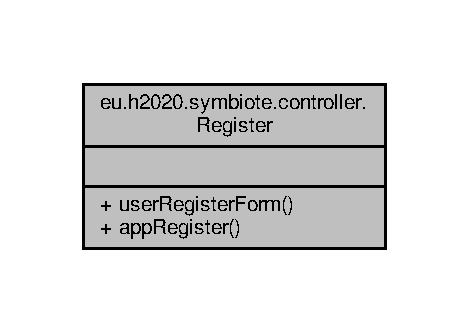
\includegraphics[width=225pt]{classeu_1_1h2020_1_1symbiote_1_1controller_1_1Register__coll__graph}
\end{center}
\end{figure}
\subsection*{Public Member Functions}
\begin{DoxyCompactItemize}
\item 
String {\bfseries user\+Register\+Form} (\hyperlink{classeu_1_1h2020_1_1symbiote_1_1model_1_1UserAccount}{User\+Account} user\+Account)\hypertarget{classeu_1_1h2020_1_1symbiote_1_1controller_1_1Register_ab996734e6e02738a0f8ee7d813c2f7cf}{}\label{classeu_1_1h2020_1_1symbiote_1_1controller_1_1Register_ab996734e6e02738a0f8ee7d813c2f7cf}

\item 
String {\bfseries app\+Register} (@Valid \hyperlink{classeu_1_1h2020_1_1symbiote_1_1model_1_1UserAccount}{User\+Account} user\+Account, Binding\+Result binding\+Result, Redirect\+Attributes redirect\+Attributes)\hypertarget{classeu_1_1h2020_1_1symbiote_1_1controller_1_1Register_af2365a11b5af23ed0c6aa32b29eb69eb}{}\label{classeu_1_1h2020_1_1symbiote_1_1controller_1_1Register_af2365a11b5af23ed0c6aa32b29eb69eb}

\end{DoxyCompactItemize}


The documentation for this class was generated from the following file\+:\begin{DoxyCompactItemize}
\item 
src/main/java/eu/h2020/symbiote/controllers/Register.\+java\end{DoxyCompactItemize}

\hypertarget{classeu_1_1h2020_1_1symbiote_1_1communication_1_1ReplyConsumer}{}\section{eu.\+h2020.\+symbiote.\+communication.\+Reply\+Consumer Class Reference}
\label{classeu_1_1h2020_1_1symbiote_1_1communication_1_1ReplyConsumer}\index{eu.\+h2020.\+symbiote.\+communication.\+Reply\+Consumer@{eu.\+h2020.\+symbiote.\+communication.\+Reply\+Consumer}}


Inheritance diagram for eu.\+h2020.\+symbiote.\+communication.\+Reply\+Consumer\+:
\nopagebreak
\begin{figure}[H]
\begin{center}
\leavevmode
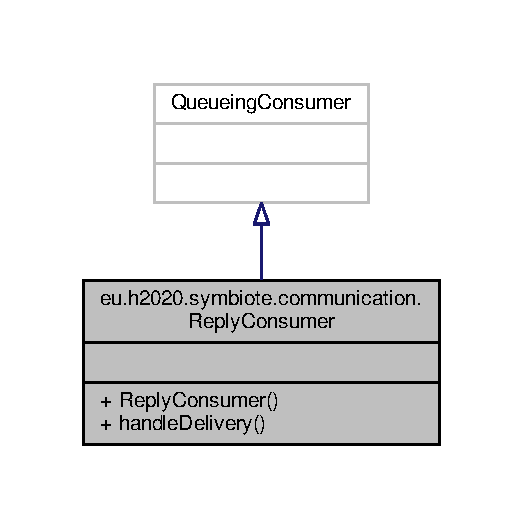
\includegraphics[width=251pt]{classeu_1_1h2020_1_1symbiote_1_1communication_1_1ReplyConsumer__inherit__graph}
\end{center}
\end{figure}


Collaboration diagram for eu.\+h2020.\+symbiote.\+communication.\+Reply\+Consumer\+:
\nopagebreak
\begin{figure}[H]
\begin{center}
\leavevmode
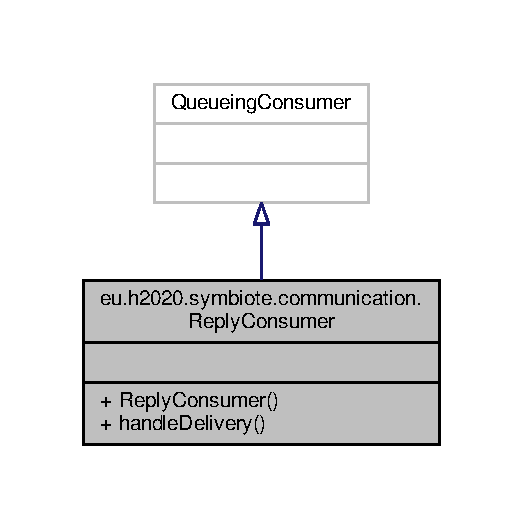
\includegraphics[width=251pt]{classeu_1_1h2020_1_1symbiote_1_1communication_1_1ReplyConsumer__coll__graph}
\end{center}
\end{figure}
\subsection*{Public Member Functions}
\begin{DoxyCompactItemize}
\item 
\hyperlink{classeu_1_1h2020_1_1symbiote_1_1communication_1_1ReplyConsumer_ac88955046a3768a0b8f83a1719ec8fa1}{Reply\+Consumer} (Channel channel, String correlation\+Id, \hyperlink{interfaceeu_1_1h2020_1_1symbiote_1_1communication_1_1IRpcResponseListener}{I\+Rpc\+Response\+Listener} response\+Listener, \hyperlink{classeu_1_1h2020_1_1symbiote_1_1communication_1_1EmptyConsumerReturnListener}{Empty\+Consumer\+Return\+Listener} empty\+Consumer\+Return\+Listener)
\item 
void \hyperlink{classeu_1_1h2020_1_1symbiote_1_1communication_1_1ReplyConsumer_a34dd66474d8fac50804af8a33642fa1d}{handle\+Delivery} (String consumer\+Tag, Envelope envelope, A\+M\+Q\+P.\+Basic\+Properties properties, byte\mbox{[}$\,$\mbox{]} body)  throws I\+O\+Exception 
\end{DoxyCompactItemize}


\subsection{Detailed Description}
R\+PC response handler. 

This class is used to consume Rabbit\+MQ response message, which comes via temporary, R\+PC response queue. 

\subsection{Constructor \& Destructor Documentation}
\index{eu\+::h2020\+::symbiote\+::communication\+::\+Reply\+Consumer@{eu\+::h2020\+::symbiote\+::communication\+::\+Reply\+Consumer}!Reply\+Consumer@{Reply\+Consumer}}
\index{Reply\+Consumer@{Reply\+Consumer}!eu\+::h2020\+::symbiote\+::communication\+::\+Reply\+Consumer@{eu\+::h2020\+::symbiote\+::communication\+::\+Reply\+Consumer}}
\subsubsection[{\texorpdfstring{Reply\+Consumer(\+Channel channel, String correlation\+Id, I\+Rpc\+Response\+Listener response\+Listener, Empty\+Consumer\+Return\+Listener empty\+Consumer\+Return\+Listener)}{ReplyConsumer(Channel channel, String correlationId, IRpcResponseListener responseListener, EmptyConsumerReturnListener emptyConsumerReturnListener)}}]{\setlength{\rightskip}{0pt plus 5cm}eu.\+h2020.\+symbiote.\+communication.\+Reply\+Consumer.\+Reply\+Consumer (
\begin{DoxyParamCaption}
\item[{Channel}]{channel, }
\item[{String}]{correlation\+Id, }
\item[{{\bf I\+Rpc\+Response\+Listener}}]{response\+Listener, }
\item[{{\bf Empty\+Consumer\+Return\+Listener}}]{empty\+Consumer\+Return\+Listener}
\end{DoxyParamCaption}
)}\hypertarget{classeu_1_1h2020_1_1symbiote_1_1communication_1_1ReplyConsumer_ac88955046a3768a0b8f83a1719ec8fa1}{}\label{classeu_1_1h2020_1_1symbiote_1_1communication_1_1ReplyConsumer_ac88955046a3768a0b8f83a1719ec8fa1}
Constructs a new instance and records its association to the passed-\/in channel.


\begin{DoxyParams}{Parameters}
{\em channel} & the channel to which this consumer is attached \\
\hline
{\em correlation\+Id} & correlation\+Id used to send R\+PC request \\
\hline
{\em response\+Listener} & listener to be notified when the response is received \\
\hline
{\em empty\+Consumer\+Return\+Listener} & listener that handles empty exchange bindings \\
\hline
\end{DoxyParams}


\subsection{Member Function Documentation}
\index{eu\+::h2020\+::symbiote\+::communication\+::\+Reply\+Consumer@{eu\+::h2020\+::symbiote\+::communication\+::\+Reply\+Consumer}!handle\+Delivery@{handle\+Delivery}}
\index{handle\+Delivery@{handle\+Delivery}!eu\+::h2020\+::symbiote\+::communication\+::\+Reply\+Consumer@{eu\+::h2020\+::symbiote\+::communication\+::\+Reply\+Consumer}}
\subsubsection[{\texorpdfstring{handle\+Delivery(\+String consumer\+Tag, Envelope envelope, A\+M\+Q\+P.\+Basic\+Properties properties, byte[] body)}{handleDelivery(String consumerTag, Envelope envelope, AMQP.BasicProperties properties, byte[] body)}}]{\setlength{\rightskip}{0pt plus 5cm}void eu.\+h2020.\+symbiote.\+communication.\+Reply\+Consumer.\+handle\+Delivery (
\begin{DoxyParamCaption}
\item[{String}]{consumer\+Tag, }
\item[{Envelope}]{envelope, }
\item[{A\+M\+Q\+P.\+Basic\+Properties}]{properties, }
\item[{byte\mbox{[}$\,$\mbox{]}}]{body}
\end{DoxyParamCaption}
) throws I\+O\+Exception}\hypertarget{classeu_1_1h2020_1_1symbiote_1_1communication_1_1ReplyConsumer_a34dd66474d8fac50804af8a33642fa1d}{}\label{classeu_1_1h2020_1_1symbiote_1_1communication_1_1ReplyConsumer_a34dd66474d8fac50804af8a33642fa1d}
Method used to handle messages coming to temporary, R\+PC response queue. 

When a new message comes to queue and the correlation ID is the same as sent in request, it is being served. It means, that if there was a response listener registered with it, it gets fired with the response delivered, and the (reply\+Queue\+Name, correlation\+ID) pair is unregistered from \hyperlink{classeu_1_1h2020_1_1symbiote_1_1communication_1_1EmptyConsumerReturnListener}{Empty\+Consumer\+Return\+Listener}.


\begin{DoxyParams}{Parameters}
{\em consumer\+Tag} & irrelevant for this implementation \\
\hline
{\em envelope} & contains routing key, which in this case is the name of temporary, R\+PC response queue \\
\hline
{\em properties} & contains correlation ID of a message to verify it\textquotesingle{}s validity \\
\hline
{\em body} & contains response to be passed to listener \\
\hline
\end{DoxyParams}

\begin{DoxyExceptions}{Exceptions}
{\em I\+O\+Exception} & \\
\hline
\end{DoxyExceptions}


The documentation for this class was generated from the following file\+:\begin{DoxyCompactItemize}
\item 
src/main/java/eu/h2020/symbiote/communication/Reply\+Consumer.\+java\end{DoxyCompactItemize}

\hypertarget{classeu_1_1h2020_1_1symbiote_1_1model_1_1RpcPlatformResponse}{}\section{eu.\+h2020.\+symbiote.\+model.\+Rpc\+Platform\+Response Class Reference}
\label{classeu_1_1h2020_1_1symbiote_1_1model_1_1RpcPlatformResponse}\index{eu.\+h2020.\+symbiote.\+model.\+Rpc\+Platform\+Response@{eu.\+h2020.\+symbiote.\+model.\+Rpc\+Platform\+Response}}


Collaboration diagram for eu.\+h2020.\+symbiote.\+model.\+Rpc\+Platform\+Response\+:
\nopagebreak
\begin{figure}[H]
\begin{center}
\leavevmode
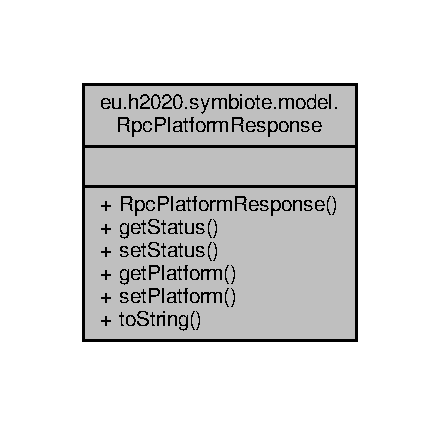
\includegraphics[width=211pt]{classeu_1_1h2020_1_1symbiote_1_1model_1_1RpcPlatformResponse__coll__graph}
\end{center}
\end{figure}
\subsection*{Public Member Functions}
\begin{DoxyCompactItemize}
\item 
\hyperlink{classeu_1_1h2020_1_1symbiote_1_1model_1_1RpcPlatformResponse_a6df0d5ad3e1f87fa68c00154c6b7eecb}{Rpc\+Platform\+Response} ()
\item 
int {\bfseries get\+Status} ()\hypertarget{classeu_1_1h2020_1_1symbiote_1_1model_1_1RpcPlatformResponse_a2b41294e25b3294f164c1387192011ec}{}\label{classeu_1_1h2020_1_1symbiote_1_1model_1_1RpcPlatformResponse_a2b41294e25b3294f164c1387192011ec}

\item 
void {\bfseries set\+Status} (int status)\hypertarget{classeu_1_1h2020_1_1symbiote_1_1model_1_1RpcPlatformResponse_ade90e8ef58f15f704ca815895826e468}{}\label{classeu_1_1h2020_1_1symbiote_1_1model_1_1RpcPlatformResponse_ade90e8ef58f15f704ca815895826e468}

\item 
\hyperlink{classeu_1_1h2020_1_1symbiote_1_1model_1_1Platform}{Platform} {\bfseries get\+Platform} ()\hypertarget{classeu_1_1h2020_1_1symbiote_1_1model_1_1RpcPlatformResponse_a52977e40eb98dedd2c2cf93033159a98}{}\label{classeu_1_1h2020_1_1symbiote_1_1model_1_1RpcPlatformResponse_a52977e40eb98dedd2c2cf93033159a98}

\item 
void {\bfseries set\+Platform} (\hyperlink{classeu_1_1h2020_1_1symbiote_1_1model_1_1Platform}{Platform} platform)\hypertarget{classeu_1_1h2020_1_1symbiote_1_1model_1_1RpcPlatformResponse_a00dfb59a3d775deb559bcb918fe37ef4}{}\label{classeu_1_1h2020_1_1symbiote_1_1model_1_1RpcPlatformResponse_a00dfb59a3d775deb559bcb918fe37ef4}

\item 
String {\bfseries to\+String} ()\hypertarget{classeu_1_1h2020_1_1symbiote_1_1model_1_1RpcPlatformResponse_aedd6526f0a148f79b9e120a21a87b96b}{}\label{classeu_1_1h2020_1_1symbiote_1_1model_1_1RpcPlatformResponse_aedd6526f0a148f79b9e120a21a87b96b}

\end{DoxyCompactItemize}


\subsection{Detailed Description}
P\+O\+JO used as a response to R\+PC call requesting platform operation. It consists of \hyperlink{classeu_1_1h2020_1_1symbiote_1_1model_1_1Platform}{Platform} object and standard H\+T\+TP status code as an integer. 

\subsection{Constructor \& Destructor Documentation}
\index{eu\+::h2020\+::symbiote\+::model\+::\+Rpc\+Platform\+Response@{eu\+::h2020\+::symbiote\+::model\+::\+Rpc\+Platform\+Response}!Rpc\+Platform\+Response@{Rpc\+Platform\+Response}}
\index{Rpc\+Platform\+Response@{Rpc\+Platform\+Response}!eu\+::h2020\+::symbiote\+::model\+::\+Rpc\+Platform\+Response@{eu\+::h2020\+::symbiote\+::model\+::\+Rpc\+Platform\+Response}}
\subsubsection[{\texorpdfstring{Rpc\+Platform\+Response()}{RpcPlatformResponse()}}]{\setlength{\rightskip}{0pt plus 5cm}eu.\+h2020.\+symbiote.\+model.\+Rpc\+Platform\+Response.\+Rpc\+Platform\+Response (
\begin{DoxyParamCaption}
{}
\end{DoxyParamCaption}
)}\hypertarget{classeu_1_1h2020_1_1symbiote_1_1model_1_1RpcPlatformResponse_a6df0d5ad3e1f87fa68c00154c6b7eecb}{}\label{classeu_1_1h2020_1_1symbiote_1_1model_1_1RpcPlatformResponse_a6df0d5ad3e1f87fa68c00154c6b7eecb}
Default empty constructor. 

The documentation for this class was generated from the following file\+:\begin{DoxyCompactItemize}
\item 
src/main/java/eu/h2020/symbiote/model/Rpc\+Platform\+Response.\+java\end{DoxyCompactItemize}

\hypertarget{classeu_1_1h2020_1_1symbiote_1_1model_1_1UserAccount}{}\section{eu.\+h2020.\+symbiote.\+model.\+User\+Account Class Reference}
\label{classeu_1_1h2020_1_1symbiote_1_1model_1_1UserAccount}\index{eu.\+h2020.\+symbiote.\+model.\+User\+Account@{eu.\+h2020.\+symbiote.\+model.\+User\+Account}}


Collaboration diagram for eu.\+h2020.\+symbiote.\+model.\+User\+Account\+:
\nopagebreak
\begin{figure}[H]
\begin{center}
\leavevmode
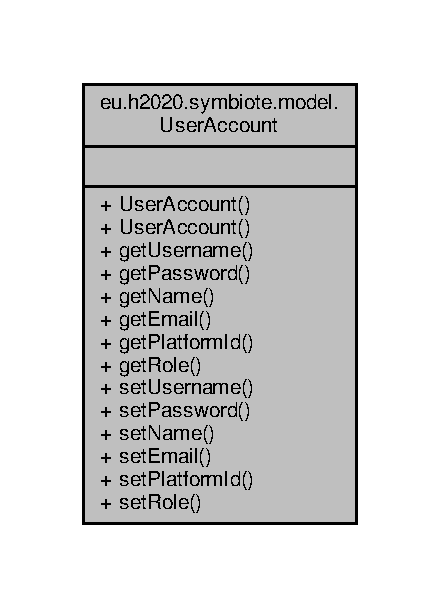
\includegraphics[width=211pt]{classeu_1_1h2020_1_1symbiote_1_1model_1_1UserAccount__coll__graph}
\end{center}
\end{figure}
\subsection*{Public Member Functions}
\begin{DoxyCompactItemize}
\item 
{\bfseries User\+Account} (String username, String password, String name, String email, int role)\hypertarget{classeu_1_1h2020_1_1symbiote_1_1model_1_1UserAccount_a1b129545cdae89fa60c0f2933f5ab2de}{}\label{classeu_1_1h2020_1_1symbiote_1_1model_1_1UserAccount_a1b129545cdae89fa60c0f2933f5ab2de}

\item 
String {\bfseries get\+Username} ()\hypertarget{classeu_1_1h2020_1_1symbiote_1_1model_1_1UserAccount_ad6495d2b5dece2369310352a6596b685}{}\label{classeu_1_1h2020_1_1symbiote_1_1model_1_1UserAccount_ad6495d2b5dece2369310352a6596b685}

\item 
String {\bfseries get\+Password} ()\hypertarget{classeu_1_1h2020_1_1symbiote_1_1model_1_1UserAccount_a13a987693380e0e8679b6aa6edfacc87}{}\label{classeu_1_1h2020_1_1symbiote_1_1model_1_1UserAccount_a13a987693380e0e8679b6aa6edfacc87}

\item 
String {\bfseries get\+Name} ()\hypertarget{classeu_1_1h2020_1_1symbiote_1_1model_1_1UserAccount_aca22562f52c72362e3cae9f5266248ba}{}\label{classeu_1_1h2020_1_1symbiote_1_1model_1_1UserAccount_aca22562f52c72362e3cae9f5266248ba}

\item 
String {\bfseries get\+Email} ()\hypertarget{classeu_1_1h2020_1_1symbiote_1_1model_1_1UserAccount_a97b599eb1aaea5a2943db5d32de43c2b}{}\label{classeu_1_1h2020_1_1symbiote_1_1model_1_1UserAccount_a97b599eb1aaea5a2943db5d32de43c2b}

\item 
String {\bfseries get\+Platform\+Id} ()\hypertarget{classeu_1_1h2020_1_1symbiote_1_1model_1_1UserAccount_a343e7b6b3497ca7260c52388ad24da93}{}\label{classeu_1_1h2020_1_1symbiote_1_1model_1_1UserAccount_a343e7b6b3497ca7260c52388ad24da93}

\item 
int {\bfseries get\+Role} ()\hypertarget{classeu_1_1h2020_1_1symbiote_1_1model_1_1UserAccount_a0d293520e72d938d1ae798603bcddaa5}{}\label{classeu_1_1h2020_1_1symbiote_1_1model_1_1UserAccount_a0d293520e72d938d1ae798603bcddaa5}

\item 
void {\bfseries set\+Username} (String username)\hypertarget{classeu_1_1h2020_1_1symbiote_1_1model_1_1UserAccount_a36810609ea028f6bc4e2480eda127725}{}\label{classeu_1_1h2020_1_1symbiote_1_1model_1_1UserAccount_a36810609ea028f6bc4e2480eda127725}

\item 
void {\bfseries set\+Password} (String password)\hypertarget{classeu_1_1h2020_1_1symbiote_1_1model_1_1UserAccount_a1cbd7fcb25d5c70f3810c08022ae4af1}{}\label{classeu_1_1h2020_1_1symbiote_1_1model_1_1UserAccount_a1cbd7fcb25d5c70f3810c08022ae4af1}

\item 
void {\bfseries set\+Name} (String name)\hypertarget{classeu_1_1h2020_1_1symbiote_1_1model_1_1UserAccount_a0a8a5622b5a96d70173c052bdef6c384}{}\label{classeu_1_1h2020_1_1symbiote_1_1model_1_1UserAccount_a0a8a5622b5a96d70173c052bdef6c384}

\item 
void {\bfseries set\+Email} (String email)\hypertarget{classeu_1_1h2020_1_1symbiote_1_1model_1_1UserAccount_af8b138dad6ec59bc1e214a87b62e57cb}{}\label{classeu_1_1h2020_1_1symbiote_1_1model_1_1UserAccount_af8b138dad6ec59bc1e214a87b62e57cb}

\item 
void {\bfseries set\+Platform\+Id} (String platform\+Id)\hypertarget{classeu_1_1h2020_1_1symbiote_1_1model_1_1UserAccount_a5a657832c8c95e42ccda3c93be6f6d2d}{}\label{classeu_1_1h2020_1_1symbiote_1_1model_1_1UserAccount_a5a657832c8c95e42ccda3c93be6f6d2d}

\item 
void {\bfseries set\+Role} (int role)\hypertarget{classeu_1_1h2020_1_1symbiote_1_1model_1_1UserAccount_ac71db7e03875310cb2dbd3e0f1d985ac}{}\label{classeu_1_1h2020_1_1symbiote_1_1model_1_1UserAccount_ac71db7e03875310cb2dbd3e0f1d985ac}

\end{DoxyCompactItemize}


The documentation for this class was generated from the following file\+:\begin{DoxyCompactItemize}
\item 
src/main/java/eu/h2020/symbiote/model/User\+Account.\+java\end{DoxyCompactItemize}

\hypertarget{classeu_1_1h2020_1_1symbiote_1_1service_1_1UserService}{}\section{eu.\+h2020.\+symbiote.\+service.\+User\+Service Class Reference}
\label{classeu_1_1h2020_1_1symbiote_1_1service_1_1UserService}\index{eu.\+h2020.\+symbiote.\+service.\+User\+Service@{eu.\+h2020.\+symbiote.\+service.\+User\+Service}}


Inheritance diagram for eu.\+h2020.\+symbiote.\+service.\+User\+Service\+:
\nopagebreak
\begin{figure}[H]
\begin{center}
\leavevmode
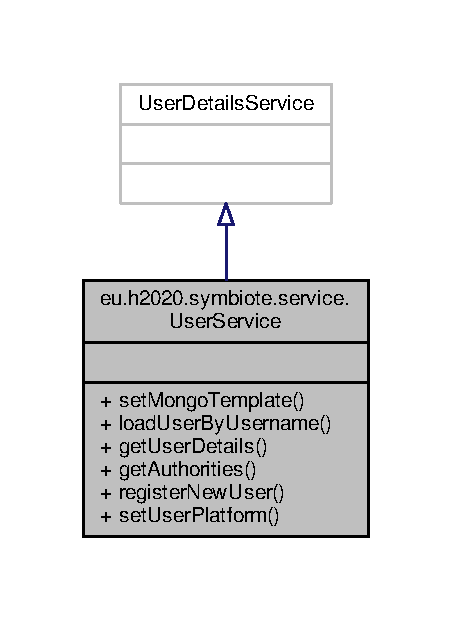
\includegraphics[width=217pt]{classeu_1_1h2020_1_1symbiote_1_1service_1_1UserService__inherit__graph}
\end{center}
\end{figure}


Collaboration diagram for eu.\+h2020.\+symbiote.\+service.\+User\+Service\+:
\nopagebreak
\begin{figure}[H]
\begin{center}
\leavevmode
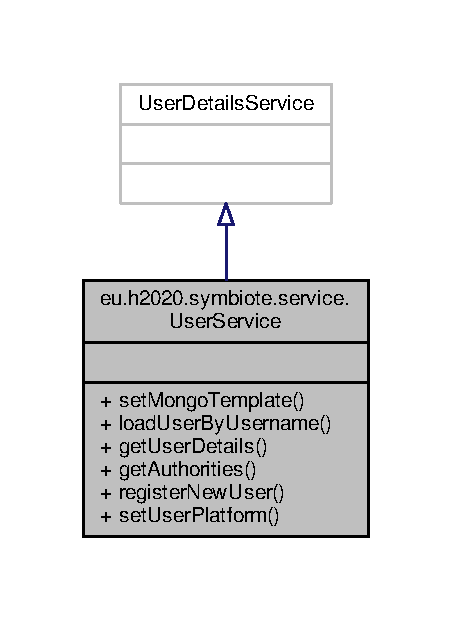
\includegraphics[width=217pt]{classeu_1_1h2020_1_1symbiote_1_1service_1_1UserService__coll__graph}
\end{center}
\end{figure}
\subsection*{Public Member Functions}
\begin{DoxyCompactItemize}
\item 
void {\bfseries set\+Mongo\+Template} (Mongo\+Template mongo\+Template)\hypertarget{classeu_1_1h2020_1_1symbiote_1_1service_1_1UserService_ad98b3b4302de53184e43943d75373a24}{}\label{classeu_1_1h2020_1_1symbiote_1_1service_1_1UserService_ad98b3b4302de53184e43943d75373a24}

\item 
User\+Details {\bfseries load\+User\+By\+Username} (String username)  throws Username\+Not\+Found\+Exception \hypertarget{classeu_1_1h2020_1_1symbiote_1_1service_1_1UserService_aa1f2db528e0aa578b24986c153d105cd}{}\label{classeu_1_1h2020_1_1symbiote_1_1service_1_1UserService_aa1f2db528e0aa578b24986c153d105cd}

\item 
\hyperlink{classeu_1_1h2020_1_1symbiote_1_1model_1_1UserAccount}{User\+Account} {\bfseries get\+User\+Details} (String username)\hypertarget{classeu_1_1h2020_1_1symbiote_1_1service_1_1UserService_a32700035211cce981b65ca042d1d1877}{}\label{classeu_1_1h2020_1_1symbiote_1_1service_1_1UserService_a32700035211cce981b65ca042d1d1877}

\item 
List$<$ Granted\+Authority $>$ {\bfseries get\+Authorities} (Integer role)\hypertarget{classeu_1_1h2020_1_1symbiote_1_1service_1_1UserService_a554976fec6b87213554328bd727ac4cb}{}\label{classeu_1_1h2020_1_1symbiote_1_1service_1_1UserService_a554976fec6b87213554328bd727ac4cb}

\item 
void {\bfseries register\+New\+User} (\hyperlink{classeu_1_1h2020_1_1symbiote_1_1model_1_1UserAccount}{User\+Account} new\+User)\hypertarget{classeu_1_1h2020_1_1symbiote_1_1service_1_1UserService_a806891ad445afc818e7a2600c275475c}{}\label{classeu_1_1h2020_1_1symbiote_1_1service_1_1UserService_a806891ad445afc818e7a2600c275475c}

\item 
void {\bfseries set\+User\+Platform} (String username, String platform\+Id)\hypertarget{classeu_1_1h2020_1_1symbiote_1_1service_1_1UserService_ac513e1a9ee5e6c750c5575a0eb775f75}{}\label{classeu_1_1h2020_1_1symbiote_1_1service_1_1UserService_ac513e1a9ee5e6c750c5575a0eb775f75}

\end{DoxyCompactItemize}


\subsection{Detailed Description}
Created by on //. 

The documentation for this class was generated from the following file\+:\begin{DoxyCompactItemize}
\item 
src/main/java/eu/h2020/symbiote/service/User\+Service.\+java\end{DoxyCompactItemize}

\hypertarget{classeu_1_1h2020_1_1symbiote_1_1WebSecurityConfig}{}\section{eu.\+h2020.\+symbiote.\+Web\+Security\+Config Class Reference}
\label{classeu_1_1h2020_1_1symbiote_1_1WebSecurityConfig}\index{eu.\+h2020.\+symbiote.\+Web\+Security\+Config@{eu.\+h2020.\+symbiote.\+Web\+Security\+Config}}


Collaboration diagram for eu.\+h2020.\+symbiote.\+Web\+Security\+Config\+:
\nopagebreak
\begin{figure}[H]
\begin{center}
\leavevmode
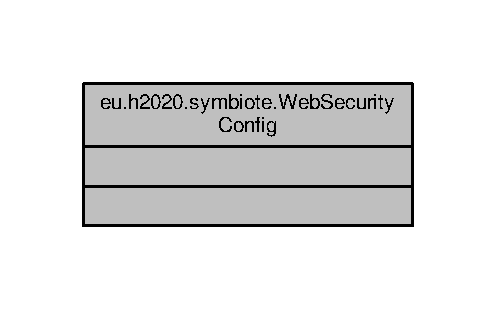
\includegraphics[width=238pt]{classeu_1_1h2020_1_1symbiote_1_1WebSecurityConfig__coll__graph}
\end{center}
\end{figure}
\subsection*{Classes}
\begin{DoxyCompactItemize}
\item 
class {\bfseries Admin\+Web\+Security\+Configurer\+Adapter}
\item 
class {\bfseries User\+Web\+Security\+Configuration\+Adapter}
\end{DoxyCompactItemize}


The documentation for this class was generated from the following file\+:\begin{DoxyCompactItemize}
\item 
src/main/java/eu/h2020/symbiote/Web\+Security\+Config.\+java\end{DoxyCompactItemize}

%--- End generated contents ---

% Index
\backmatter
\newpage
\phantomsection
\clearemptydoublepage
\addcontentsline{toc}{chapter}{Index}
\printindex

\end{document}
